%!TEX root = ../dissertation.tex

% Evaluation
\section{Evaluation}
\label{sec:evaluation}
Our main goal is to obtain basic statistical values that allow us to decide which deployment
approach is more suitable to fulfill the requirements of smart place applications based on \gls{RFID}
technology. The evaluation process will compare the approaches in regard to low-latency and will
evaluate the data storage performance for the Fosstrak platform.

% Present the evaluation methodology for both cases
\subsection{Evaluation Methodology}
\label{sub:eval_methodology}
In order to determine which deployment approach is more adequate to meet the latency requirements and to
evaluate the data storage performance for the Fosstrak platform, we propose the following
methodologies:

% Evaluation Methodologies : Latency
\subsubsection{Latency Interaction}
\label{sub:eval_methodology_latency}
The response time between an event that occurs in the smart warehouse and the corresponding action
that is triggered in the physical space, the proposed methodology consists in perform the monitoring
of the smart warehouse network and determine how much time is spent between the \gls{ALE} collect the
event triggered and client application receive the notification report, as illustrated in
Figure~\ref{fig:eval_latency_methodology}.

% Latency Interaction Evaluation Methodology Figure
\begin{figure}[ht!]
  \centering
  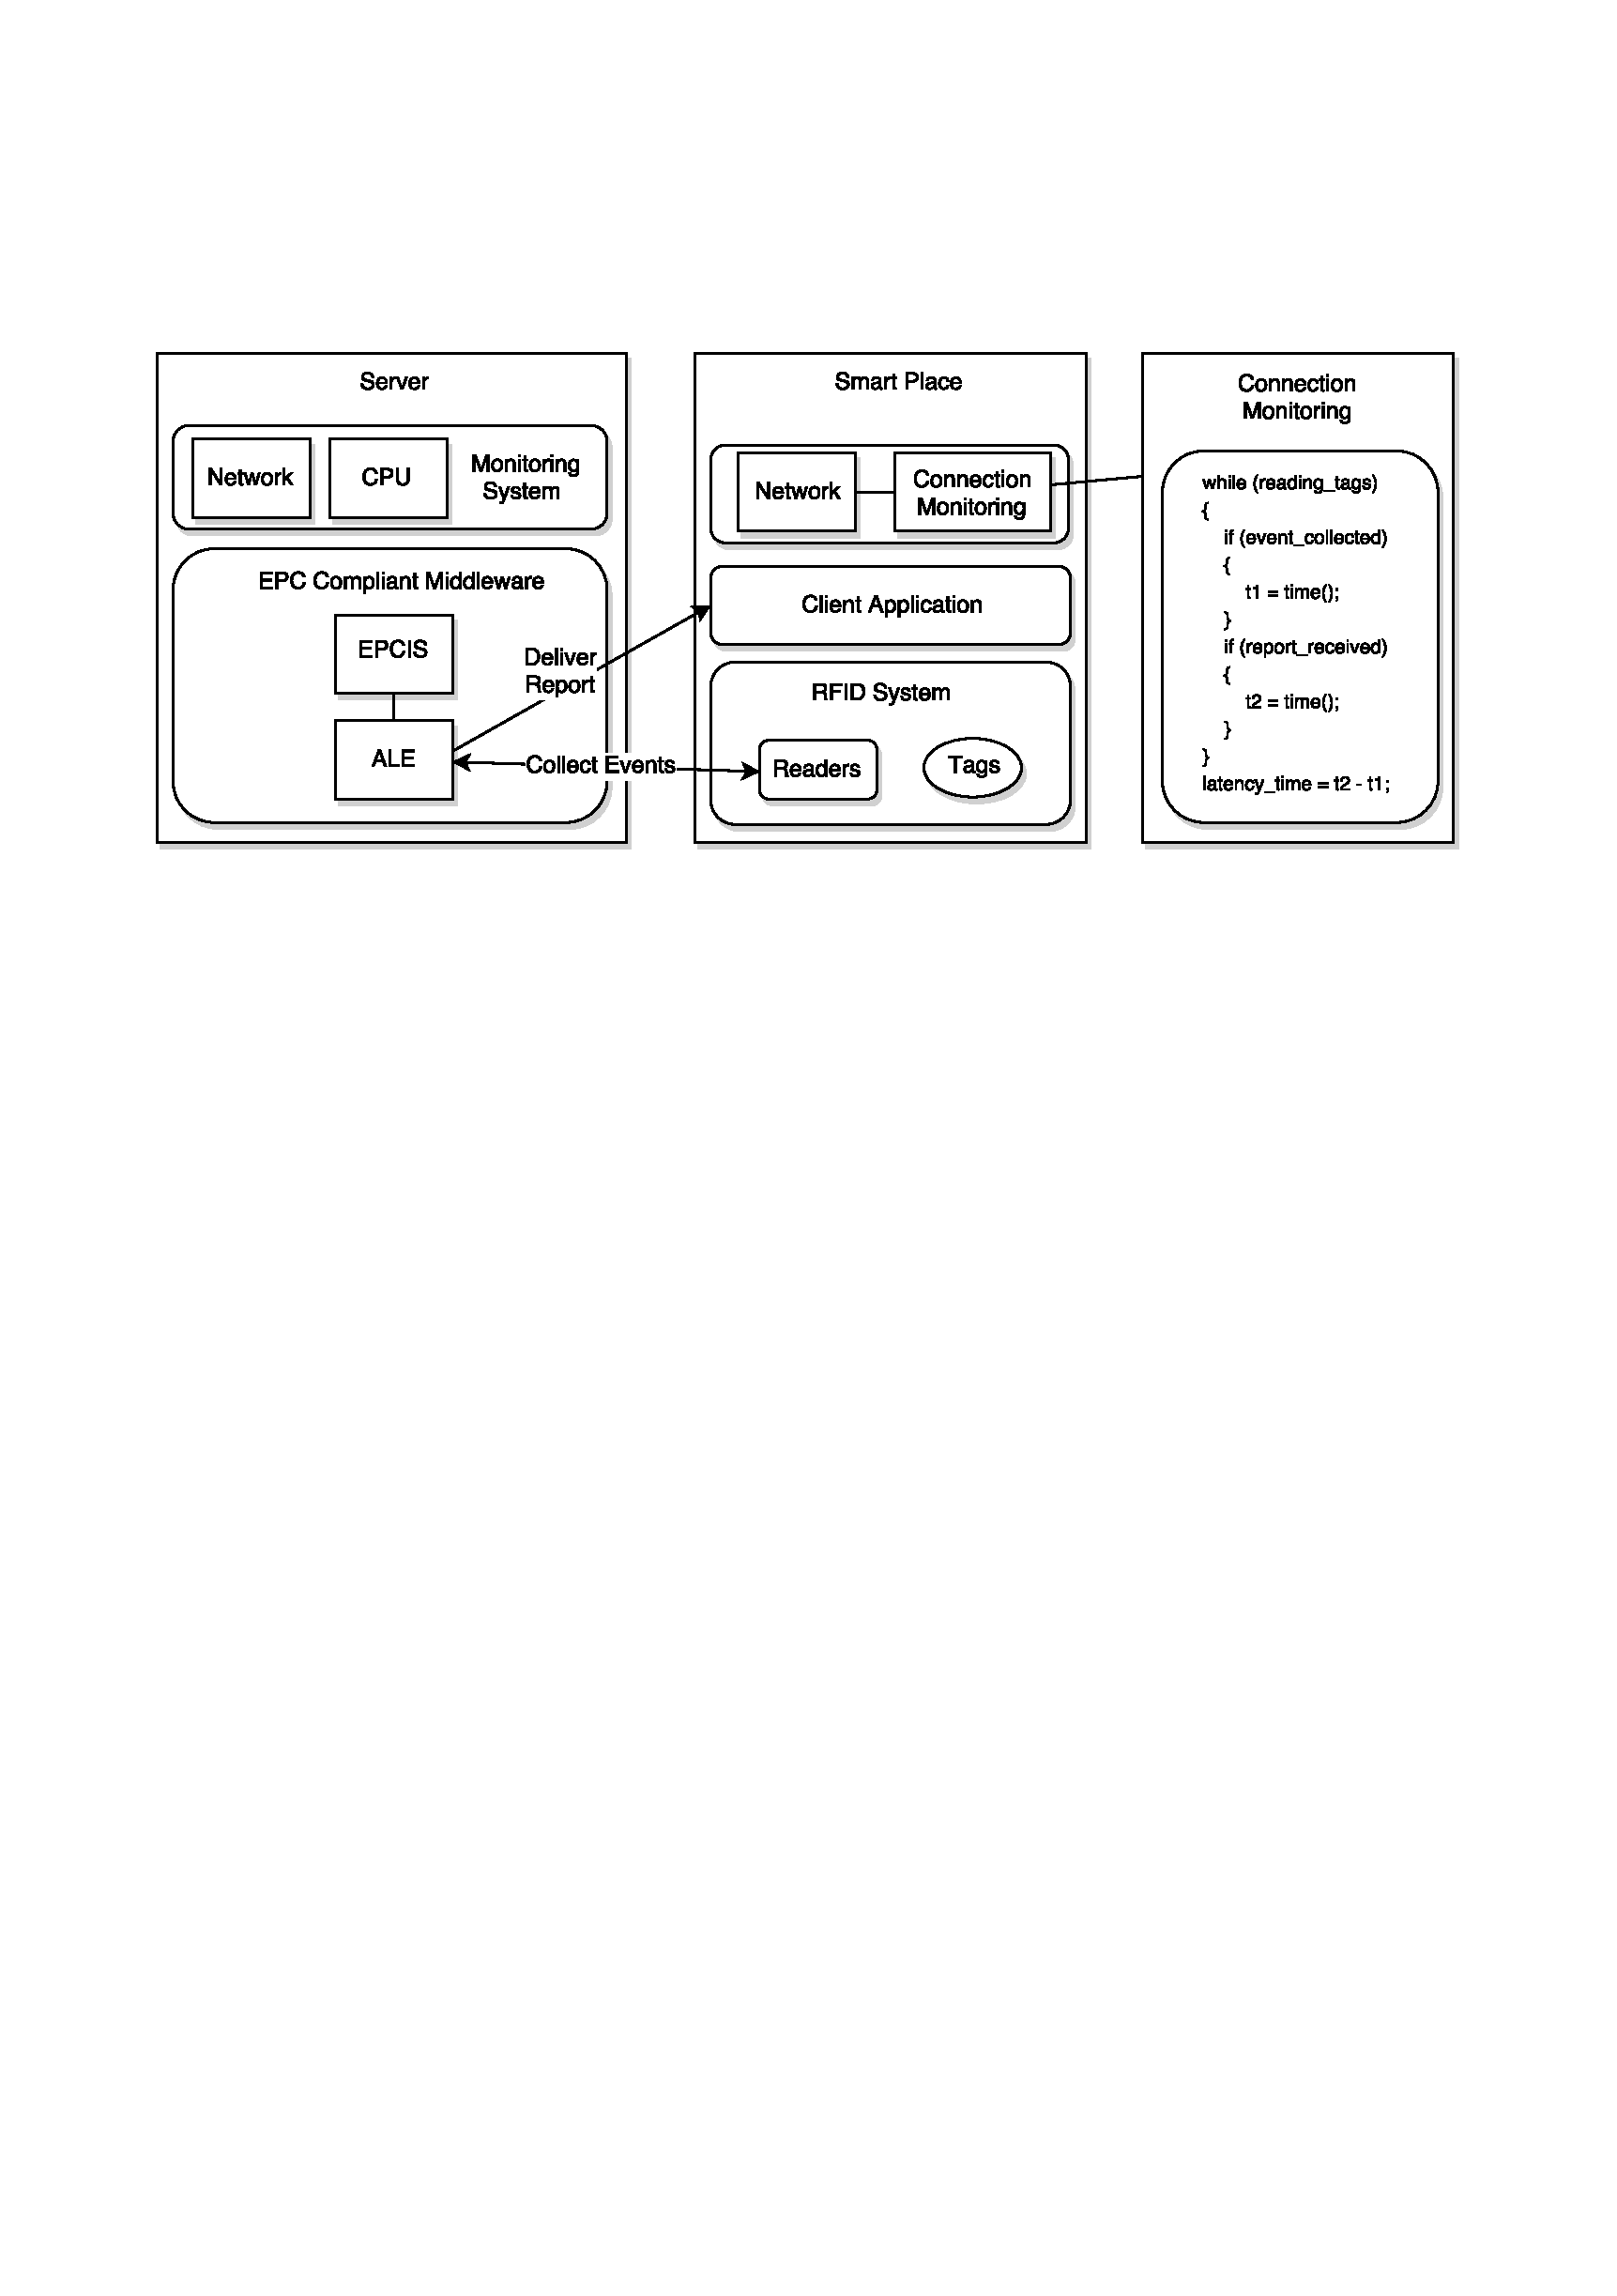
\includegraphics[width=.5\textwidth]{./figures/eval_latency_methodology}
  \caption[Latency evaluation methodology.]{Latency interaction evaluation methodology.}
  \label{fig:eval_latency_methodology}
\end{figure}

The \gls{ALE} module is responsible for collecting and processing the reader events and take the
correct decisions based on those events. In the Fosstrak implementation the collection and processing
of reader events is performed according to an \textit{Event Cycle} specification. The \textit{Event Cycle}
is a set of periodical cycles where the \gls{ALE} module collect the events from the readers. The data
about the \textit{Event Cycle} is delivered to the client application through a report. The information
in the report can be used to notify the client regarding an event in the smart warehouse or even to
trigger a new event in the warehouse such as open or close a door.

The smart warehouse is running a monitoring system that stores information about the incoming and outgoing
packets in the warehouse network. The Fosstrak \gls{ALE} module can be configured to generate
information to register when a new event is processed and also when a new report is delivered to the
client. Thus, with the information provided by the monitoring system and the \gls{ALE} module it is
possible to calculate the latency request for an event that occurs in the warehouse. The warehouse network
connection was monitored with the \textit{tcpdump}\footnote{\url{http://www.tcpdump.org/}}, a command-line
tool that allows the monitoring of the packets that are being transmitted or received over a network.
Through the logs produced by this tool, we are able to determine how the connection time is spent.

With this methodology we intend to obtain information regarding how the communication time is spent
when an event is triggered in the warehouse for the deployment approaches described in Section~\ref{sec:solution}.
In order to determine which approach is more adequate to deploy the application, we defined a set of
metrics that will allow us to compare the performance of the fog-based and cloud-based deployment
approaches and help to determine which one is more adequate to deploy the smart warehouse
application.

% Evaluation Methodologies : Data
\subsubsection{Data Storage Performance}
To evaluate the data storage performance for a RFID application based on Fosstrak, the proposed
methodology consists in stress the EPCIS Repository by simulating several readers that are concurrently
triggering events - through HTTP requests - to the repository that is running in the cloud. This
simulation was performed through JMeter\footnote{http://jmeter.apache.org/}, a Java application
designed to perform load testing and measure application performance. We will analyze how is the
behavior for some performance metrics such as \textit{CPU Utilization} and the volume of incoming
network traffic (\textit{Network In}).

% Evaluation Setup
\subsection{Evaluation Setup}
\label{sub:eval_setup}
To perform the evaluation experiments we chose \gls{AWS} as cloud provider. All the experiments were
conducted in \gls{AWS} \gls{EC2} instances running the Amazon Linux \gls{AMI} operating system. The \glspl{VM}
presents a configuration with a 2.5 \textit{\gls{GHz}} single-core processor with 1 \textit{\gls{GB}} of
\gls{RAM}. In the fog-approach configuration, the experiments were conducted in a \gls{VM} with
a 2.6 \textit{\gls{GHz}} dual-core processor with 2 \textit{\gls{GB}} of \gls{RAM} and running
the \textit{Linux Ubuntu 14.04.2 LTS} operating system. The smart warehouse was connected to the cloud
and fog through a \gls{ADSL} connection with a bandwidth of 10 Mbps.

Regarding the software components, the application stack is composed of the \textit{Apache Tomcat 7.0.52.0}\footnote{\url{http://tomcat.apache.org/}}
with \textit{Java} version \textit{1.7.0} update \textit{79}. The \gls{RFID} middleware used was the Fosstrak
(described in section \ref{sub:fosstrak}) and the versions were: \textit{a) \gls{FCServer}} version
\textit{1.2.0}; \textit{b) Capture Application} version \textit{0.1.1}; and \textit{c) \gls{EPCIS} Repository}
version \textit{0.5.0}. Furthermore, the \gls{EPCIS} Repository was connected to a \textit{MySQL server}
version \textit{5.5}. The Rifidi Emulator\footnote{\url{http://rifidi.org}} used to emulate the \gls{RFID}
readers is in version \textit{1.6.0}.

% Performed Experiments
\subsection{Experiments Performed}
\label{sub:eval_experiments}
The experiments performed in our evaluation were based on the scenario and data from the RFIDToys \cite{Correia:Thesis:2014}
Master Thesis. In short, the RFIDToys is a warehouse demonstrator consisting of a robot transporting
tagged products that are identified by RFID readers deployed in the physical space. In the
performed experiments, we use a scenario where a tagged robot was programmed to execute
a given number of laps in the warehouse plant where exists an automatic door that
opens when one of the RFID readers that are placed in the plant detects that the robot is
approaching.

\subsubsection{Latency Interaction}
\label{subs:eval_exp_latency}
To evaluate the latency interaction according the methodology proposed in Section~\ref{sub:eval_methodology_latency},
During the lap the robot stops during 5 seconds in front of the door and then continues its lap.
The door must be opened before the robot starts to moving again. To perform the simulation we defined
two different specifications (\textit{ECspec}) for the \textit{Event Cycles} of the \gls{ALE} module,
\textit{Baseline Event Cycle} and \textit{Half-period Event Cycle}. The configuration parameters
for the \textit{ECspecs} are presented in Table~\ref{table:ecspec_parameters}.

% ECspec parameters
\begin{table}[ht!]
 \begin{tabular}{|l|c|c|c|}
  \hline
  Event Cycle Specification & Period  & Duration & Iterations  \\ \hline
  Baseline Event Cycle      &  10s    & 9.5s     & 10          \\ \hline
  Half-period Event Cycle   &   5s    & 4.75s    & 20          \\ \hline
 \end{tabular}
 \caption[Event Cycle parameters.]{Event Cycle parameters.}
 \label{table:ecspec_parameters}
\end{table}

The evaluation of the event latency for the proposed approaches was performed in two steps. First,
we want to determine during a \textit{Event Cycle} how much time the \gls{ALE} is processing an event
and how much time the module is in an idle state. Furthermore, we want to determine how much time
each stage of the event processing pipeline takes. To achieve that we proposed the following metrics
based on the event processing pipeline stages: (i) \textit{Upload Time}; (ii) \textit{Tag Processing Time};
(iii) \textit{Filtering \& Aggregation Time}; (iv) \textit{Report Creation Time}; and finally (v)
\textit{Response Time}.

% Cloud-based warehouse latency
\subsubsection{Cloud-based warehouse latency}
\label{subs:eval_exp_latency_ecspec_fast}
The behavior expected when the \gls{ALE} is configured with a faster \textit{Event Cycle} specification
is that the event latency presents a better overall performance. According the obtained results it is possible
to observe that the event latency decrease from 8.244s to 4.266s. The values for the network latency
improved when the \gls{ALE} is configured with the faster \textit{ECspec}, close to $\approx65\%$ of
improvement for the \textit{Upload Time} metric - from 0.294s to 0.103s - and $\approx40\%$ for the
\textit{Response Time} metric - from 0.228s to 0.149s. The values for the time where the \gls{ALE}
remains in an idle state also presented a significant improvement, from 7.346s to 2.569s. The value
for the \textit{Tag Processing Time} increased $\approx1000\%$ when the \gls{ALE} is configured with
\textit{Half-period ECspec} - from 0.002s to 0.024s. The value for the \textit{Filtering \& Aggregation Time}
metric increased $\approx300\%$ - from 0.370s to 1.490s.

% Event Time Breakdown
\textit{a) Event Time Breakdown.}
In the current experiment the \gls{ALE} module was configured with the \textit{Baseline ECspec} and
the \textit{Half-period ECspec}.

% Baseline ECspec event time breakdown
\begin{figure}[ht!]
  \centering
  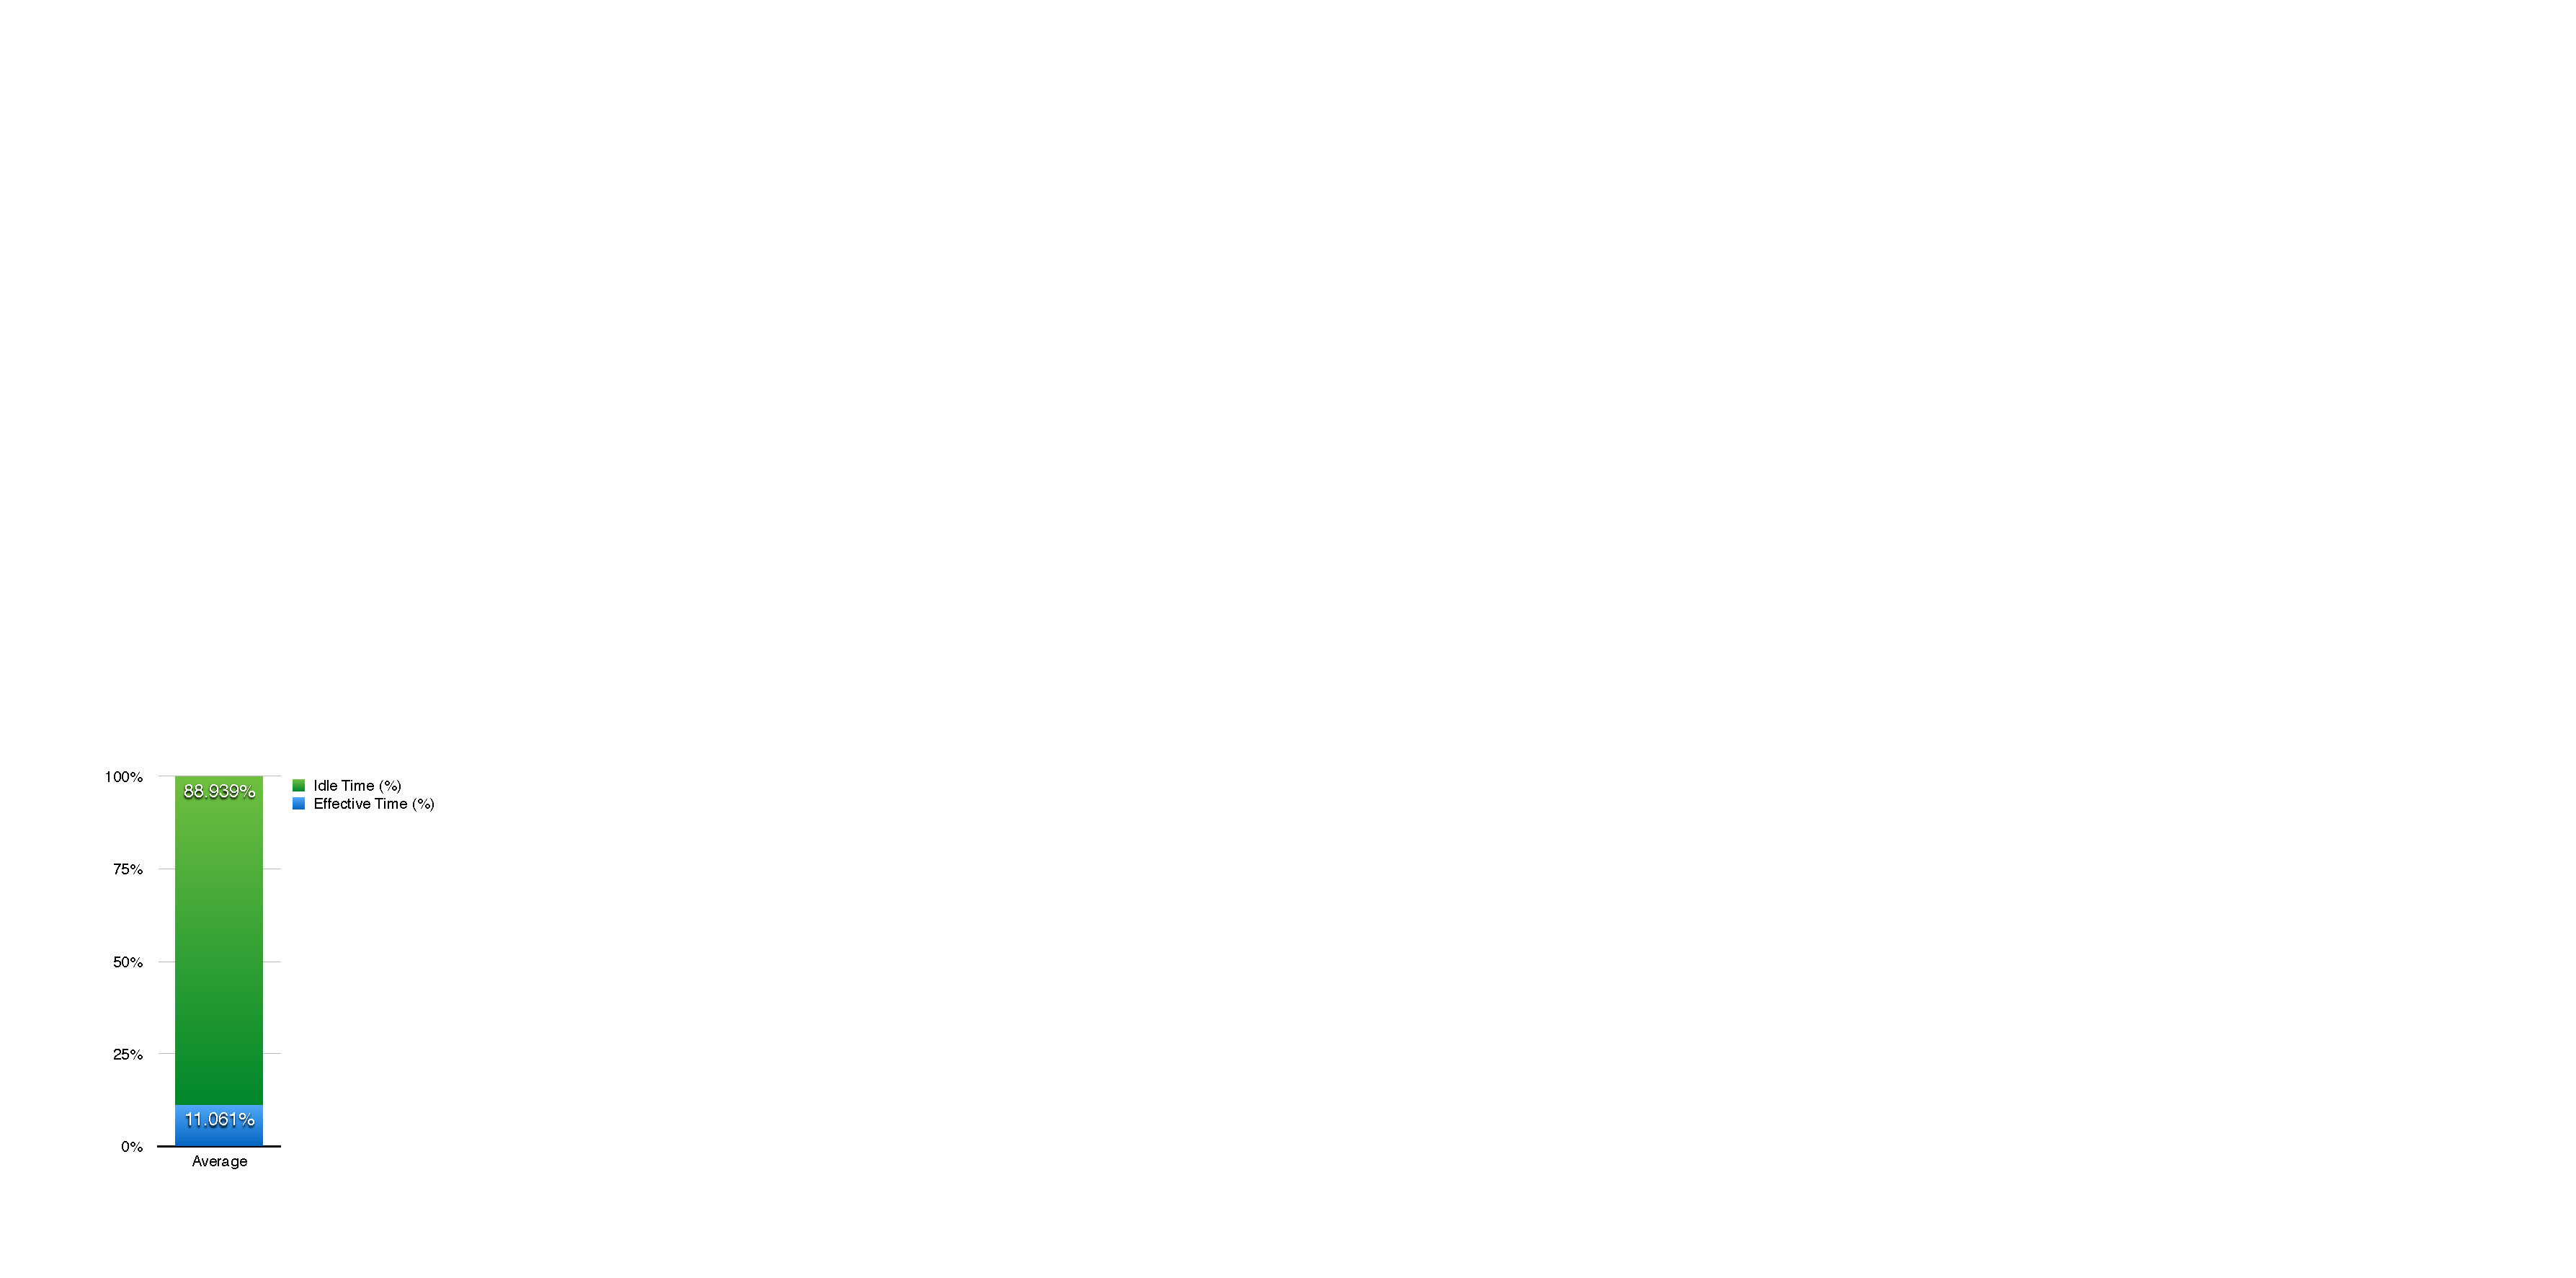
\includegraphics[width=.55\linewidth]{./figures/cloud_ecspec_breakdown}
  \caption{Baseline Event Cycle: latency breakdown.}
  \label{fig:ecspecf_base}
\end{figure}

% ECSpec fast cloud breakdown figure
\begin{figure}[ht!]
  \centering
  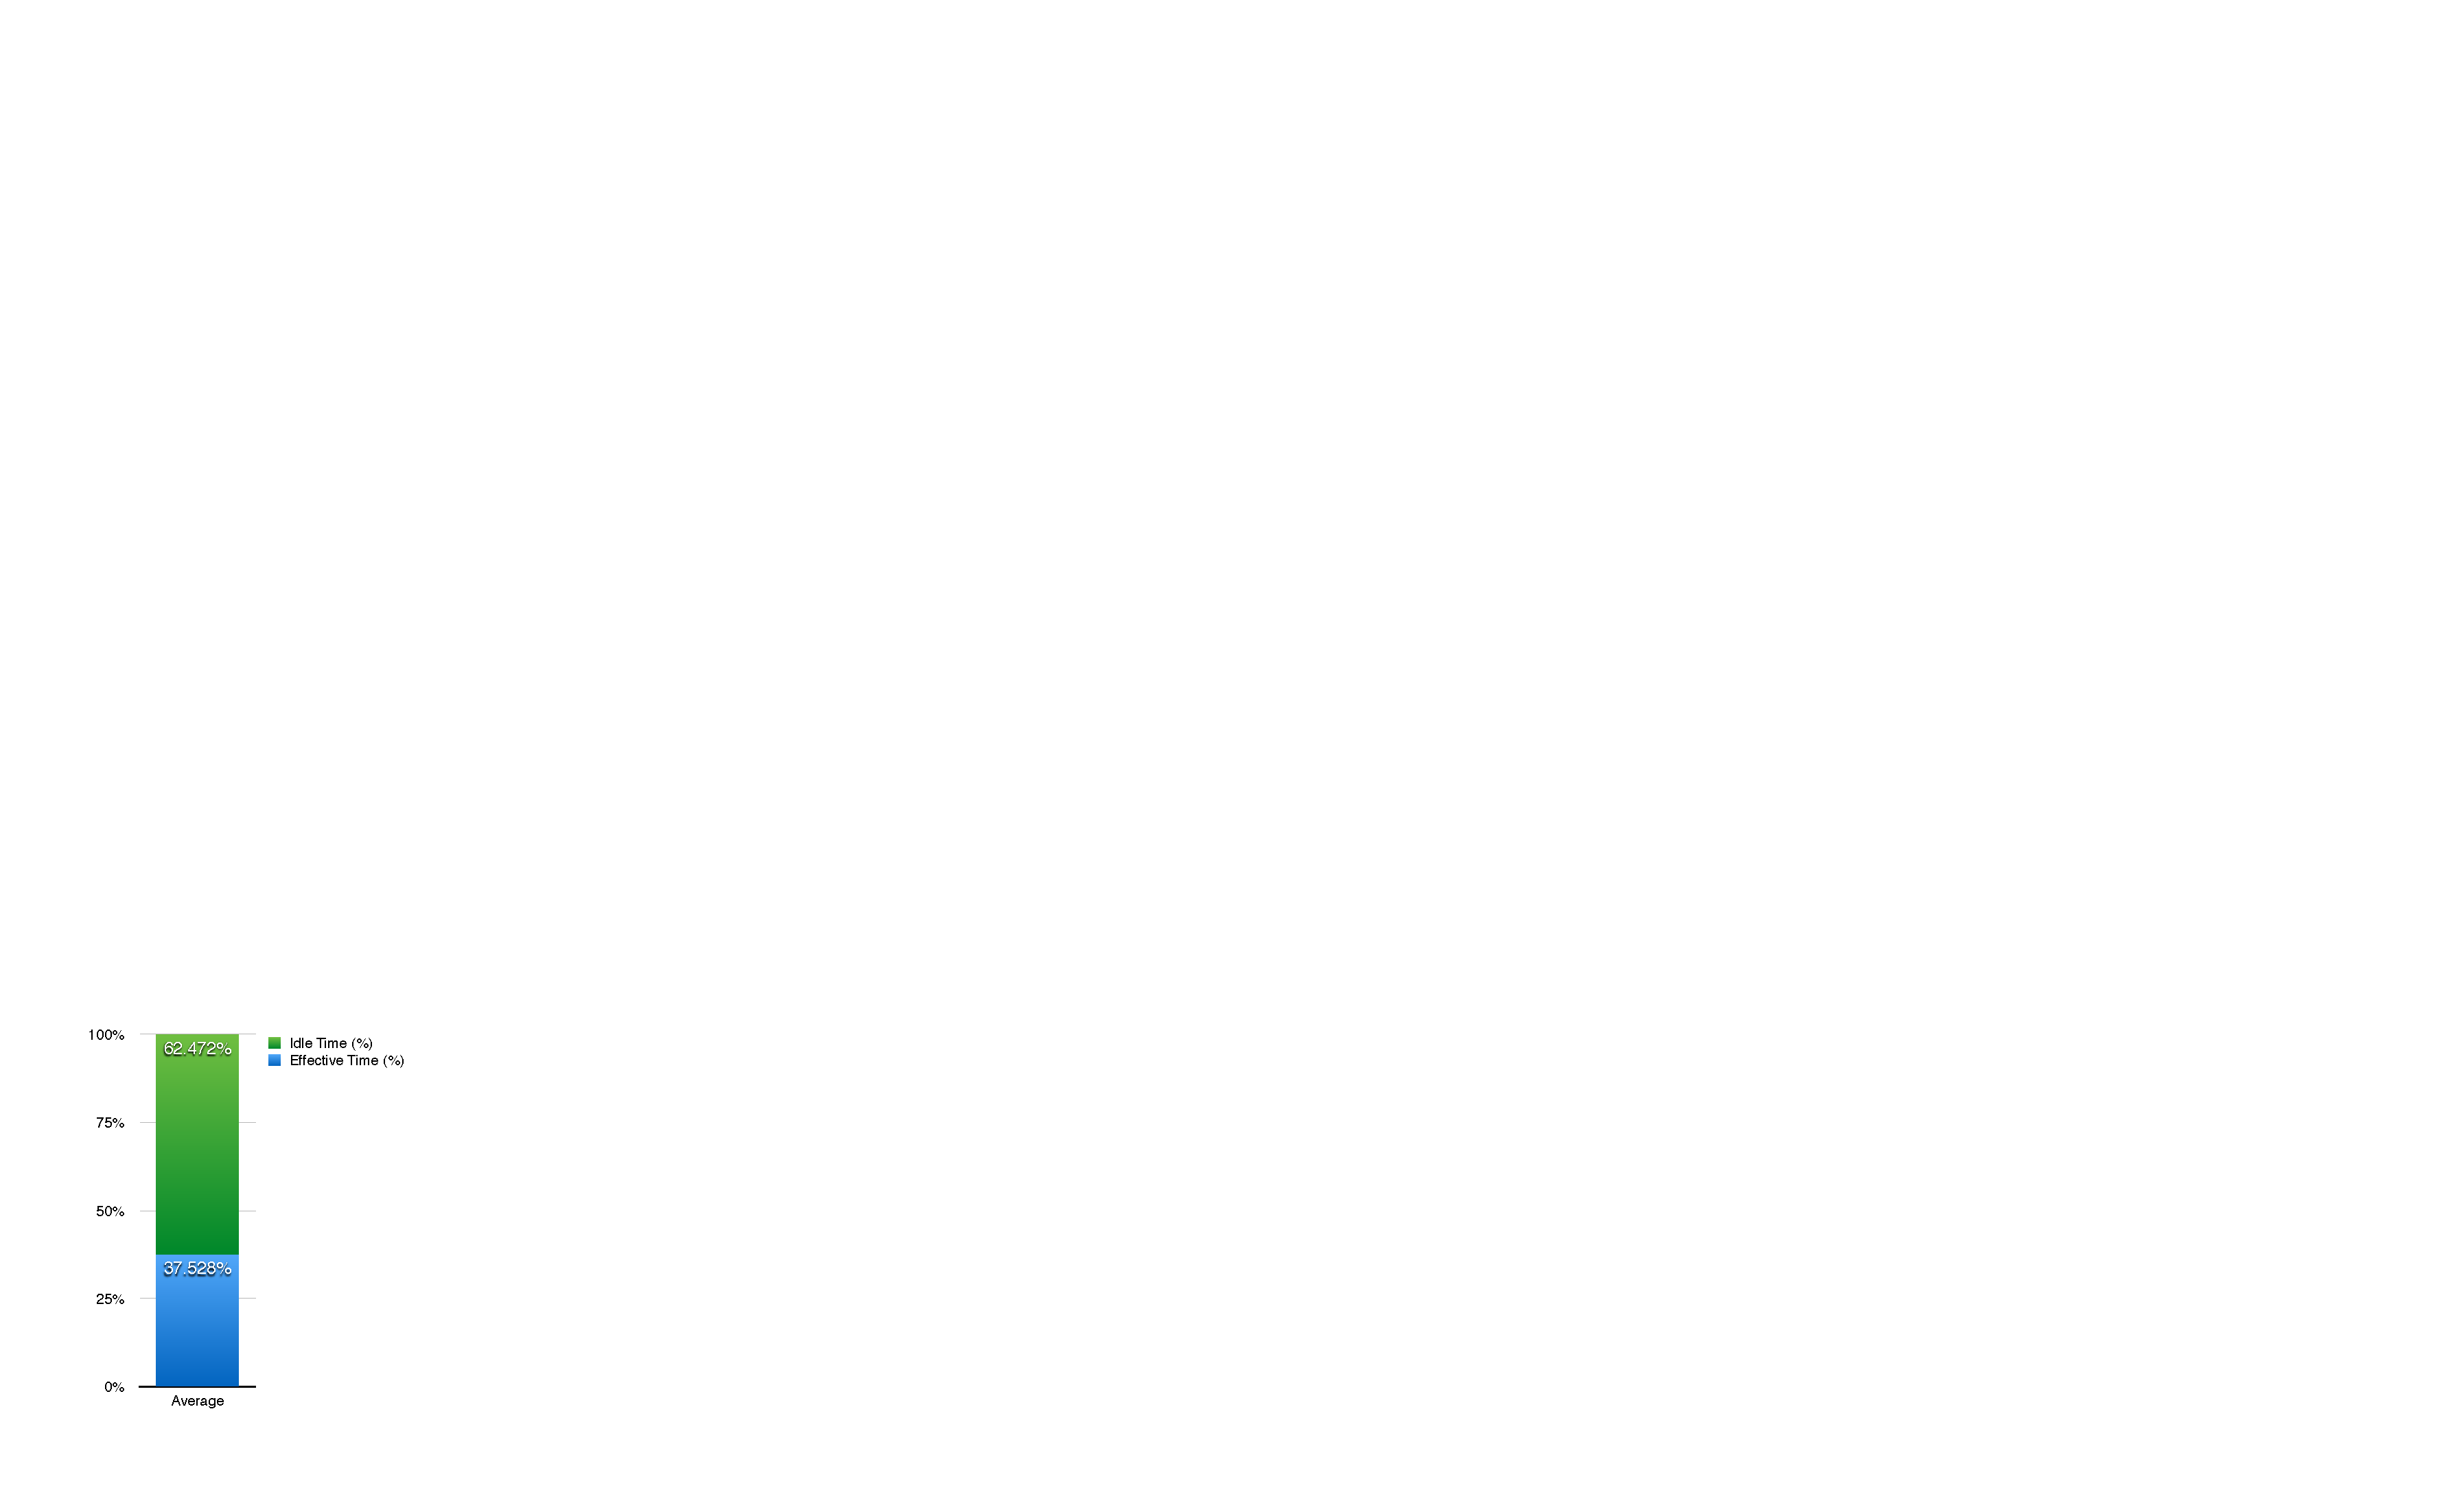
\includegraphics[width=.55\linewidth]{./figures/cloud_ecspecf_breakdown}
  \caption{Half-period Event Cycle: latency breakdown.}
  \label{fig:ecspecf_half}
\end{figure}

The graphs presented in Figure~\ref{fig:ecspecf_base} and Figure~\ref{fig:ecspecf_half} show that,
during most of time of an \textit{Event Cycle} the \gls{ALE} module is in an idle state.
Also, it is possible to observe that the \textit{ECspecs} affected the percentage of time where
\gls{ALE} is processing the events (\textit{Effective Time}) and where is in an idle state (\textit{Idle Time}).
With the \textit{Baseline ECspec} the \gls{ALE} remains $\approx89\%$ of the \textit{Event Cycle} period
in an idle state while when configured with the \textit{Half-period ECspec} this value decreases to
$\approx62\%$. This means that during the \textit{Event Cycle} period the \gls{ALE} module can be in
an idle state during 9 seconds when configured with the \textit{Baseline ECspec} while with the
\textit{Half-period ECspec} this value can last for 3 seconds.

% Event Effective Time Breakdown
\textit{b) Event Effective Time Breakdown.}
Figure~\ref{fig:ecspecf_effective_base} presents the how much time is spent in each phase of
the pipeline when the \gls{ALE} is configured with \textit{Baseline ECspec} and in
Figure~\ref{fig:ecspecf_effective_half} when it is configured with the \textit{Half-period ECspec}.

% ECSpec Fast local breakdown figure
\begin{figure}[ht!]
  \centering
  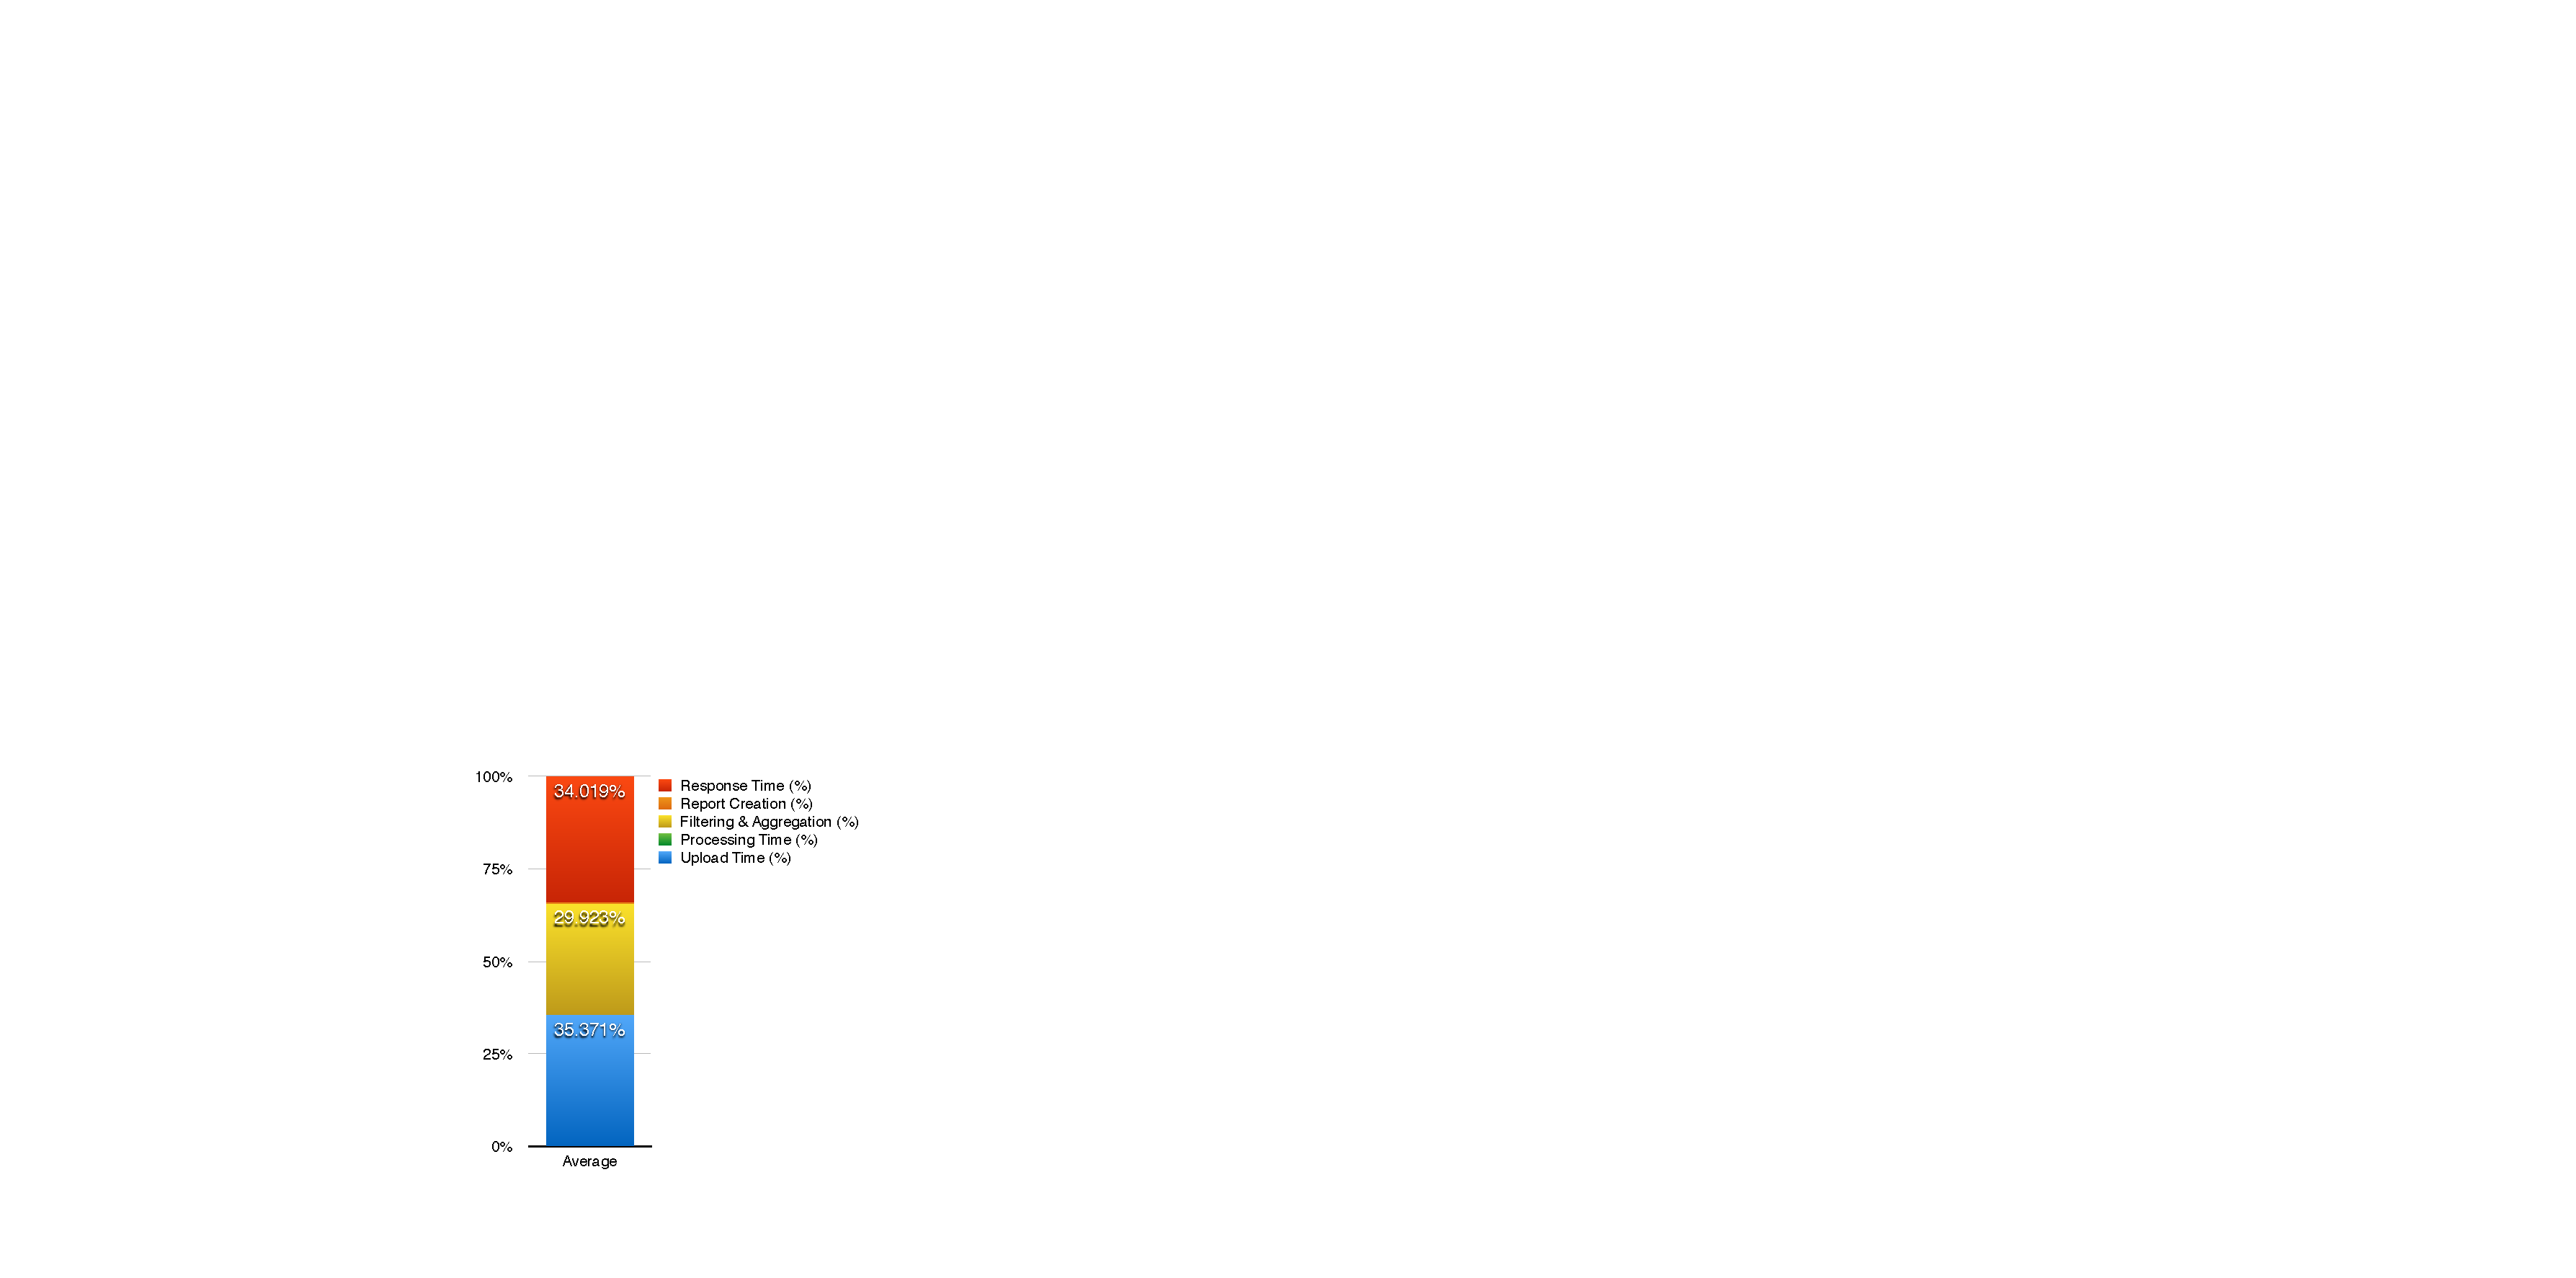
\includegraphics[width=.7\linewidth]{./figures/cloud_ecspec_effective_breakdown}
  \caption{Baseline Event Cycle: event pipeline breakdown.}
  \label{fig:ecspecf_effective_base}
\end{figure}

% ECSpec fast cloud breakdown figure
\begin{figure}[ht!]
  \centering
  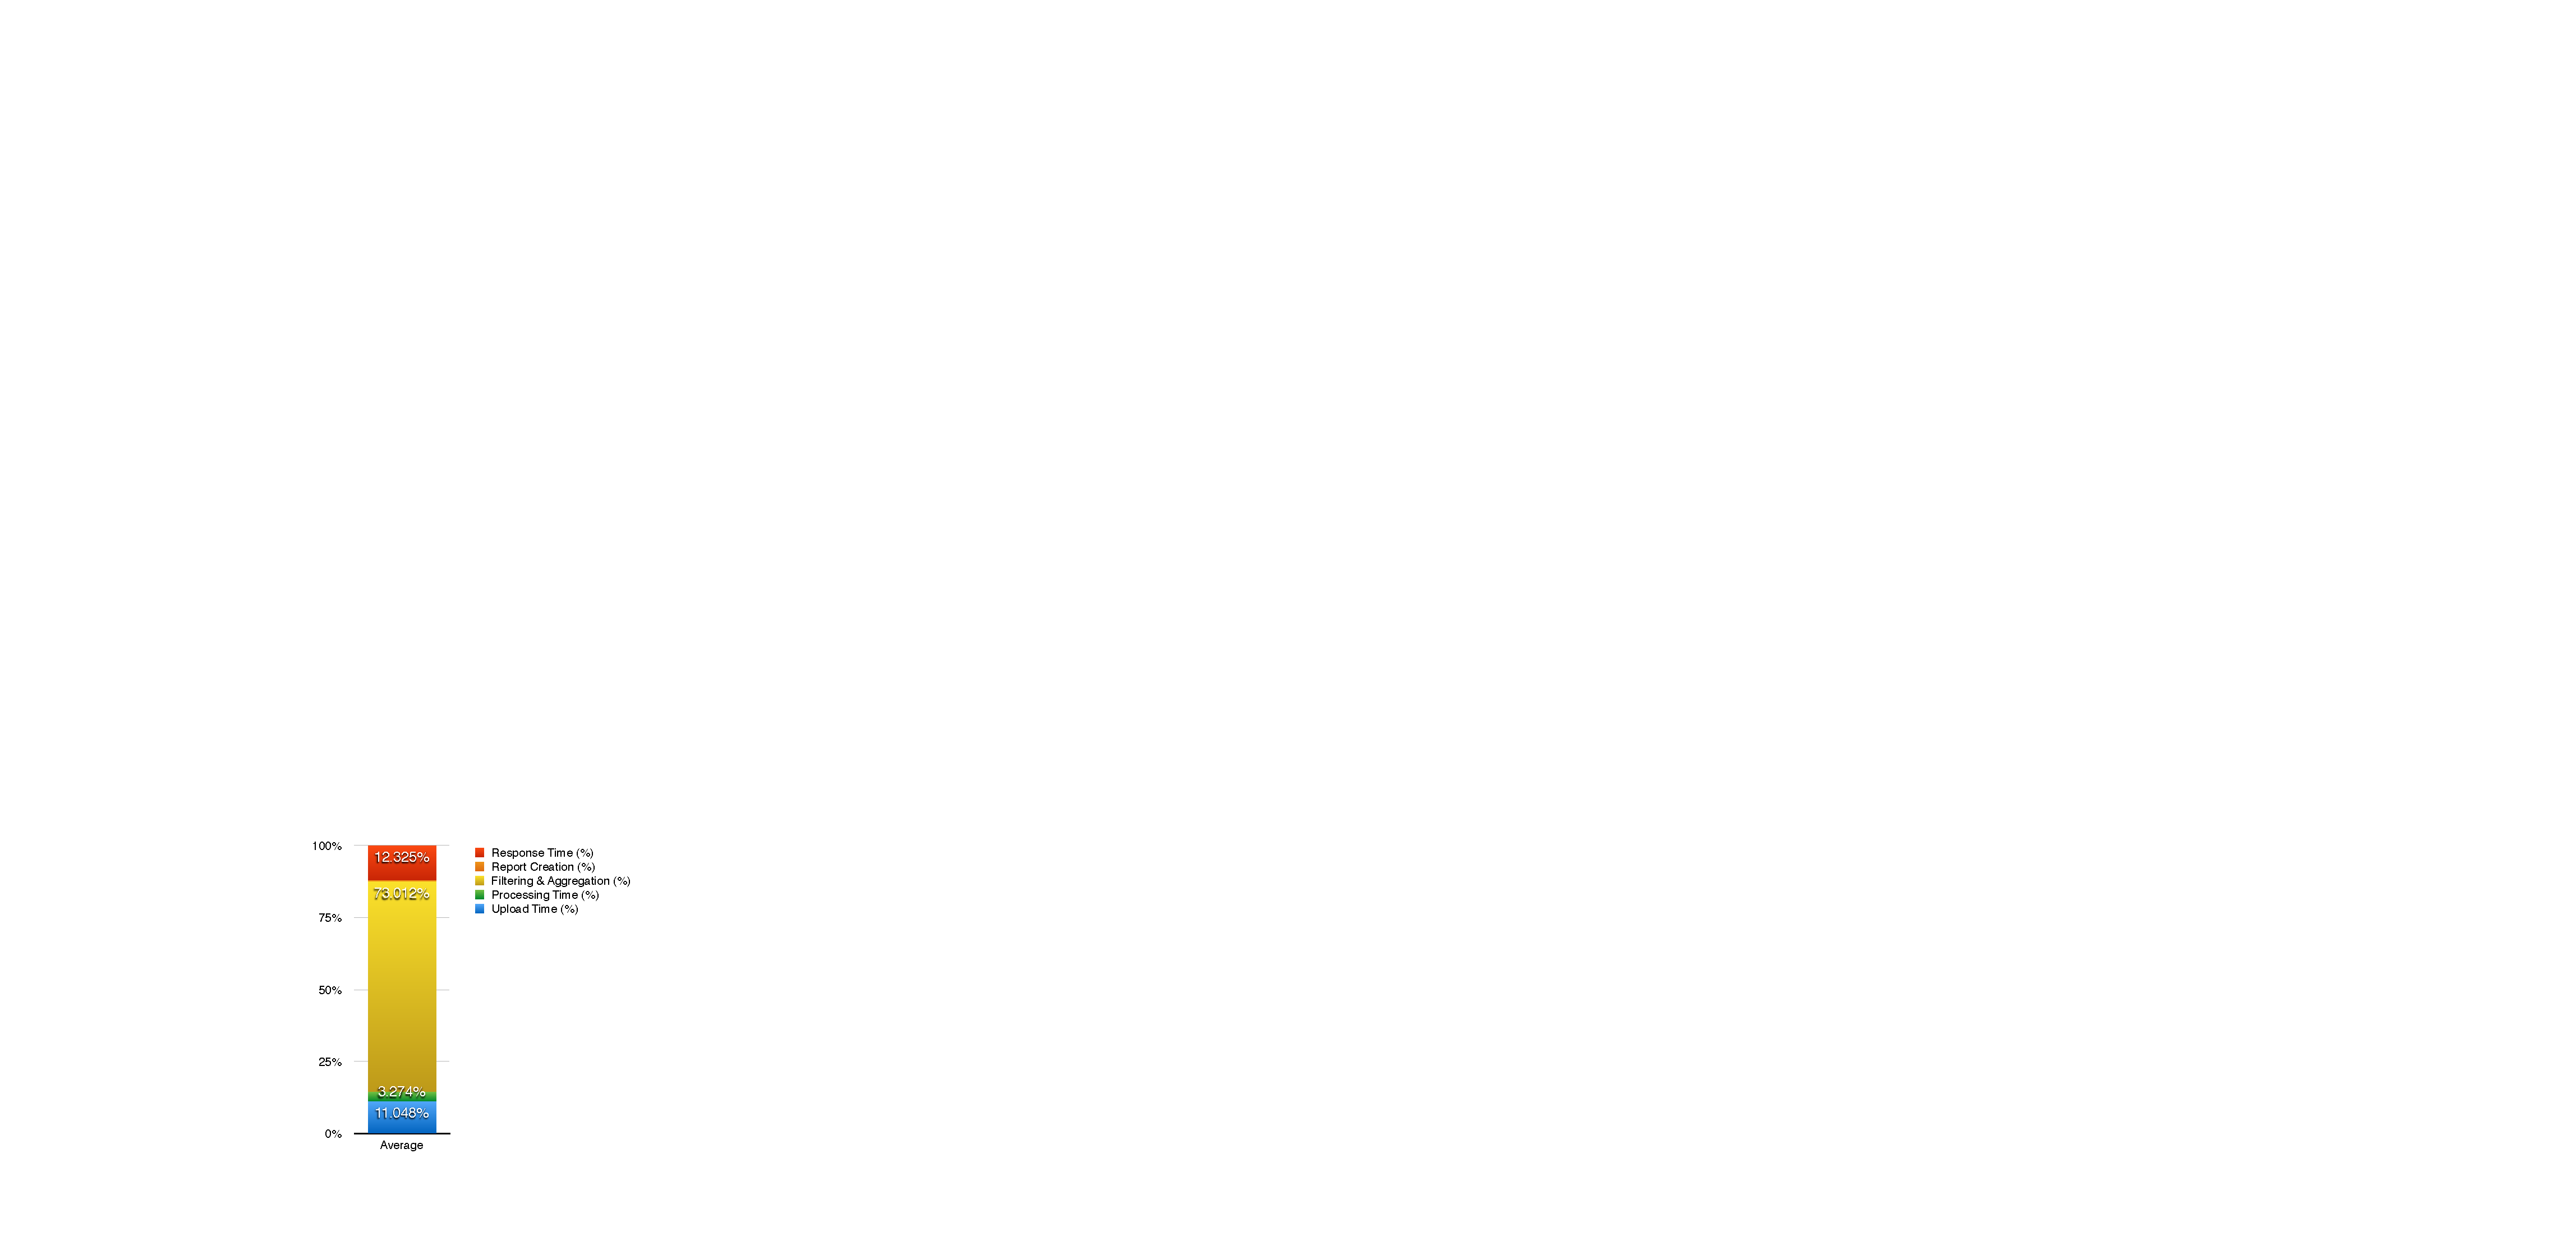
\includegraphics[width=.7\linewidth]{./figures/cloud_ecspecf_effective_breakdown}
  \caption{Half-period Event Cycle: event pipeline breakdown.}
  \label{fig:ecspecf_effective_half}
\end{figure}

Comparing the obtained results, it is possible to observe that time breakdown is evenly distributed
between the \textit{Upload} ($\approx35\%$), \textit{Filtering \& Aggregation} ($\approx30\%$) and
\textit{Response} ($\approx34\%$) stages when the \gls{ALE} module is configured with the \textit{Baseline ECspec},
while the \textit{Tag Processing} and \textit{Report Creation} stages represents a small percentage of the
total time, less than $\approx1\%$. When the \gls{ALE} is configured with the \textit{Half-period ECspec},
the \textit{Filtering \& Aggregation} stage is the most time consuming, representing close to $\approx 73\%$
of the total time. As when configured with the \textit{Baseline ECspec}, the \textit{Upload} and
\textit{Response} stages presents similar results, respectively close to $\approx11\%$ and $\approx12\%$.
Regarding the \textit{Processing} stage, the time required to process the event data increased in a significant
way, from less than $\approx0.3\%$ to $\approx3\%$. The \textit{Report Creation} stage presented the same
values from the \textit{Baseline ECspec} configuration ($\approx0.3\%$).

% Experiment Result
\textit{c) Experiment Result.}
In our scenario, that means the warehouse door only will open if the \gls{ALE} module was configured
with the \textit{Half-period ECspec}, otherwise the robot will crash with the door.

% Fog-based warehouse latency
\subsubsection{Fog-based warehouse latency}
\label{subs:eval_exp_latency_ecspec}
As in the previous experiment the event latency presented a better overall performance for the
faster \textit{ECspec}. According the obtained values we observed that the event latency improves
in a significant way - from 7.450s to 4.250s. This result is achieved thanks to the improvement in
the latency of at the \textit{Filtering \& Aggregation Time} by $\approx52\%$ - from 2.530s to 1.230s -
and the amount of time that \gls{ALE} is in an idle state - from 4.944s to 2.747s. Regarding the
network latency, the values for the \textit{Upload Time} and \textit{Response Time} improved 1ms
for both metrics. However, when configured with a faster \textit{Event Cycle} specification the
tag processing time presented an inferior performance, where time to process the event data increases
$\approx470\%$ - from 0.049s to 0.279s. Also the report creation time increased $300\%$ - from 0.001s to 0.003s.

% Event Time Breakdown
\textit{a) Event Time Breakdown.}
Figure~\ref{fig:ecspec_base} shows the latency breakdown for an event when the \gls{ALE} module is
configured with the \textit{Baseline ECspec} and in Figure~\ref{fig:ecspec_half} when it is configured
with the \textit{Half-period ECspec}.

% ECSpec breakdown figure
\begin{figure}[ht!]
 \centering
 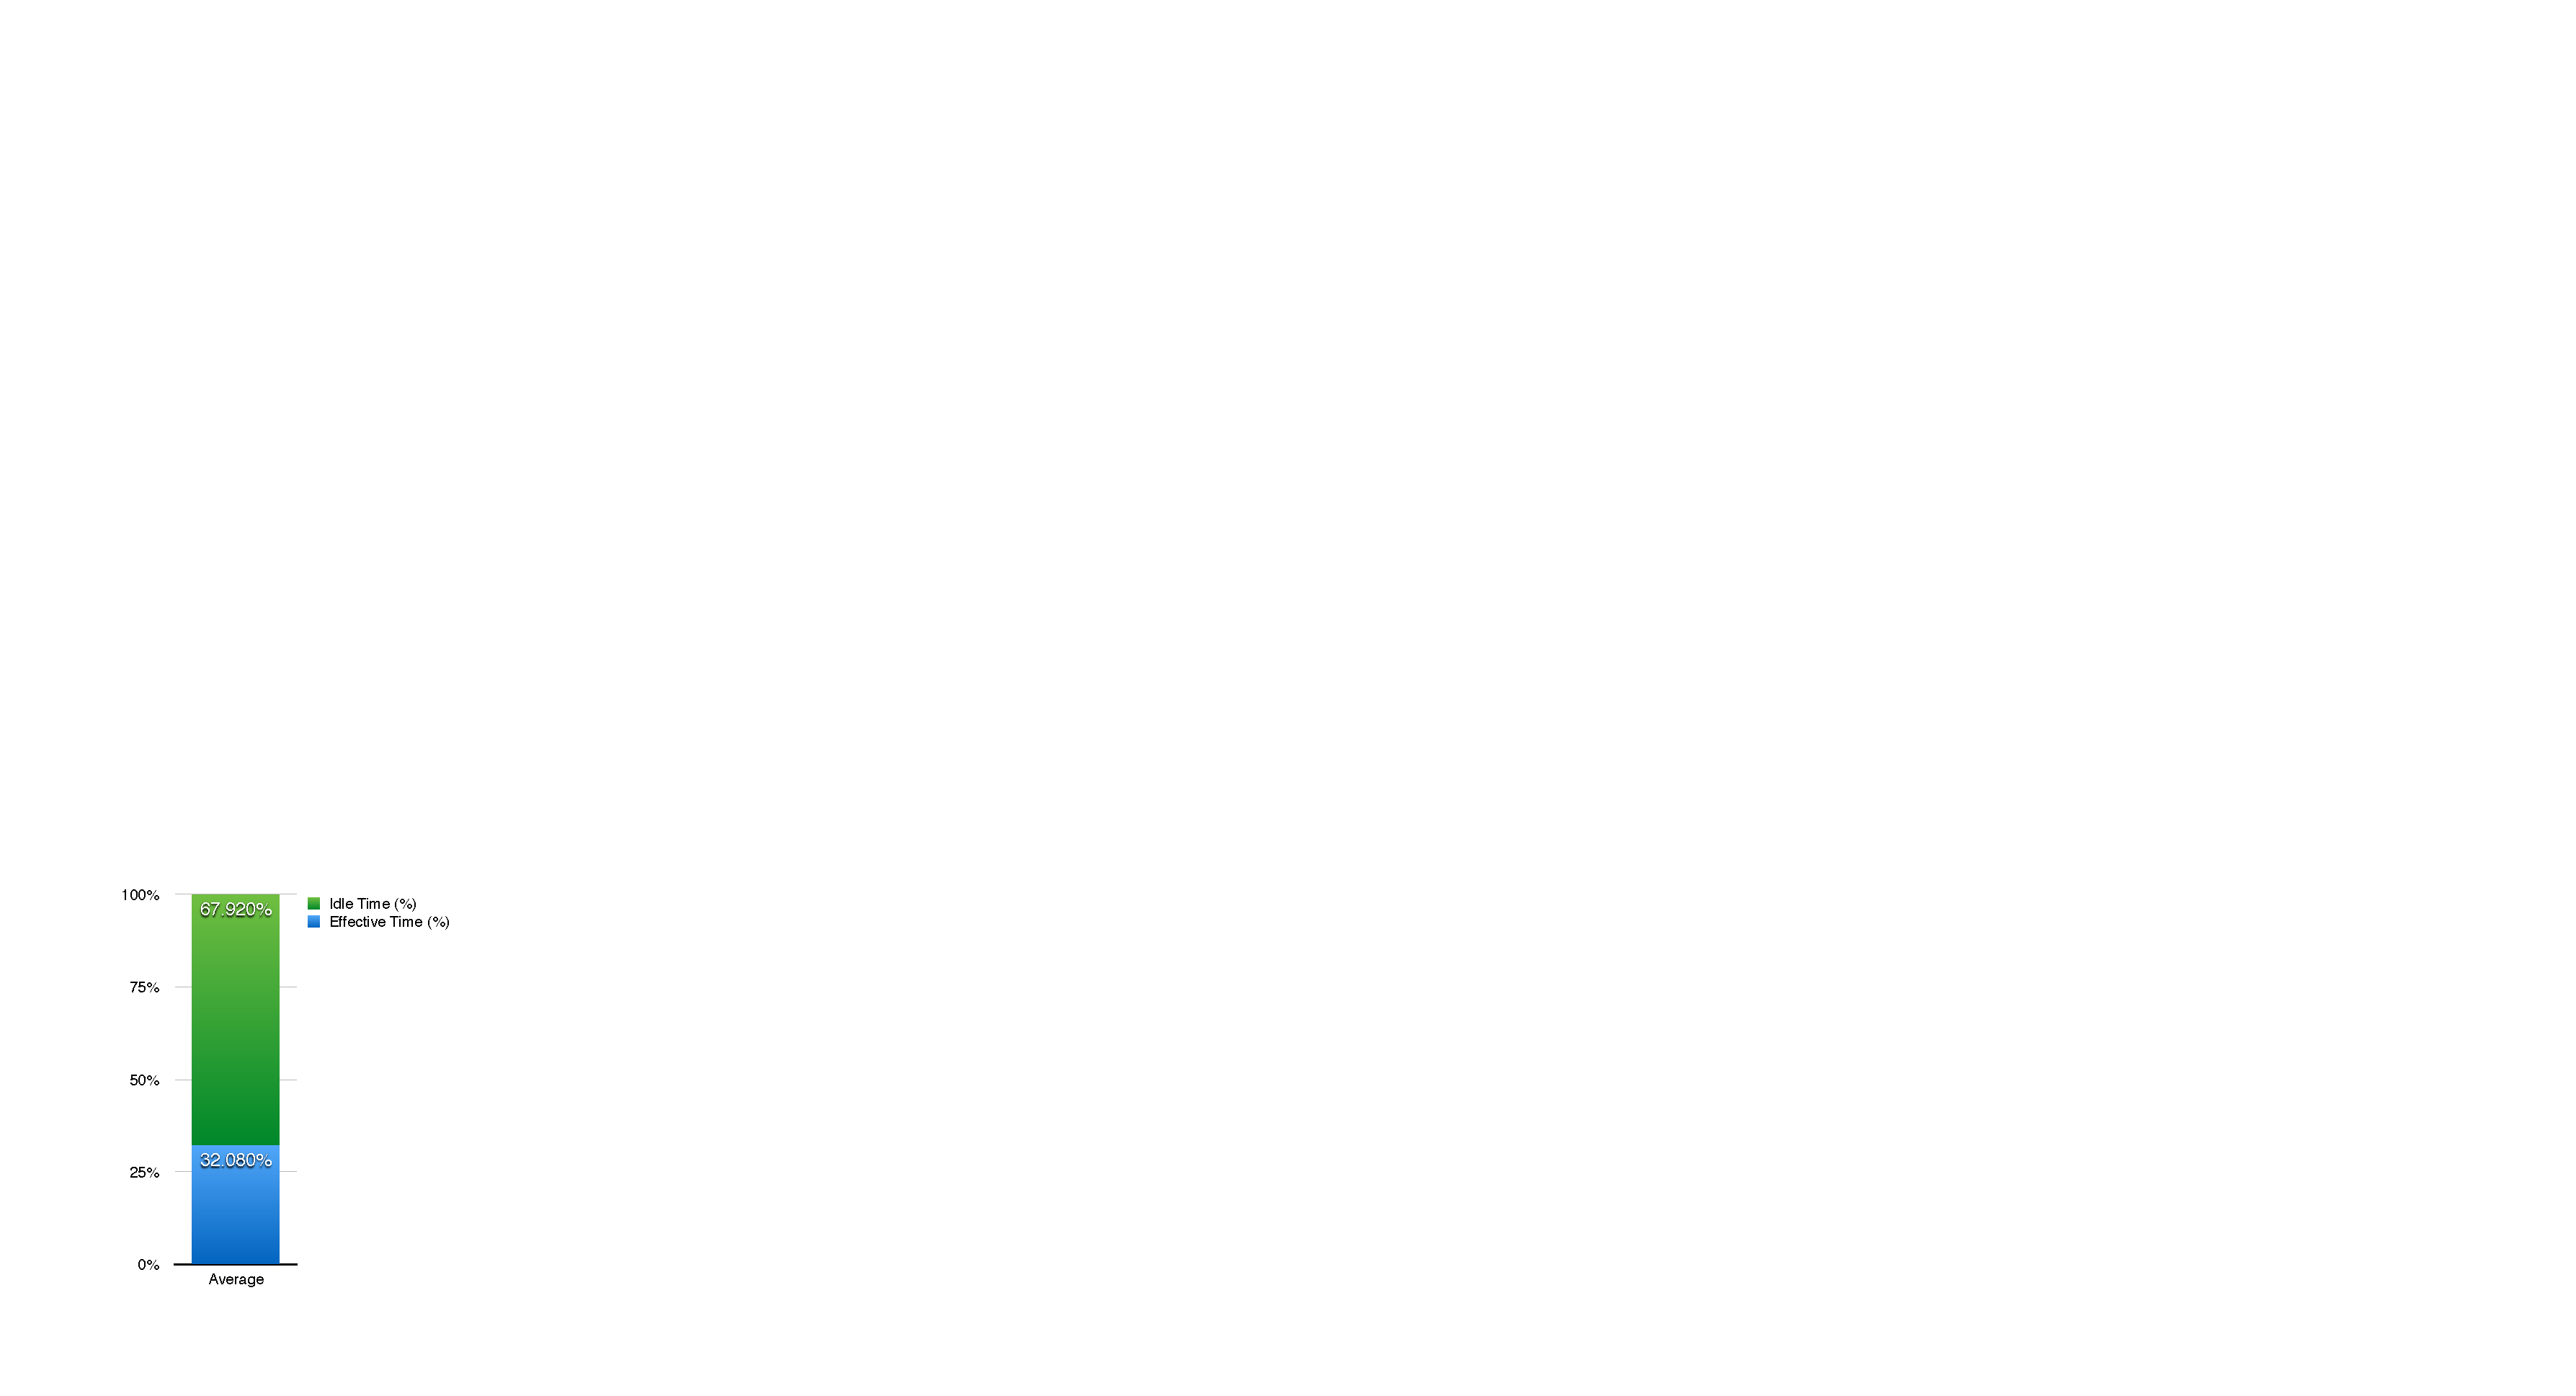
\includegraphics[width=.55\linewidth]{./figures/edge_ecspec_breakdown}
 \caption{Baseline Event Cycle: latency breakdown.}
 \label{fig:ecspec_base}
\end{figure}

% ECSpec fast breakdown figure
\begin{figure}[ht!]
 \centering
 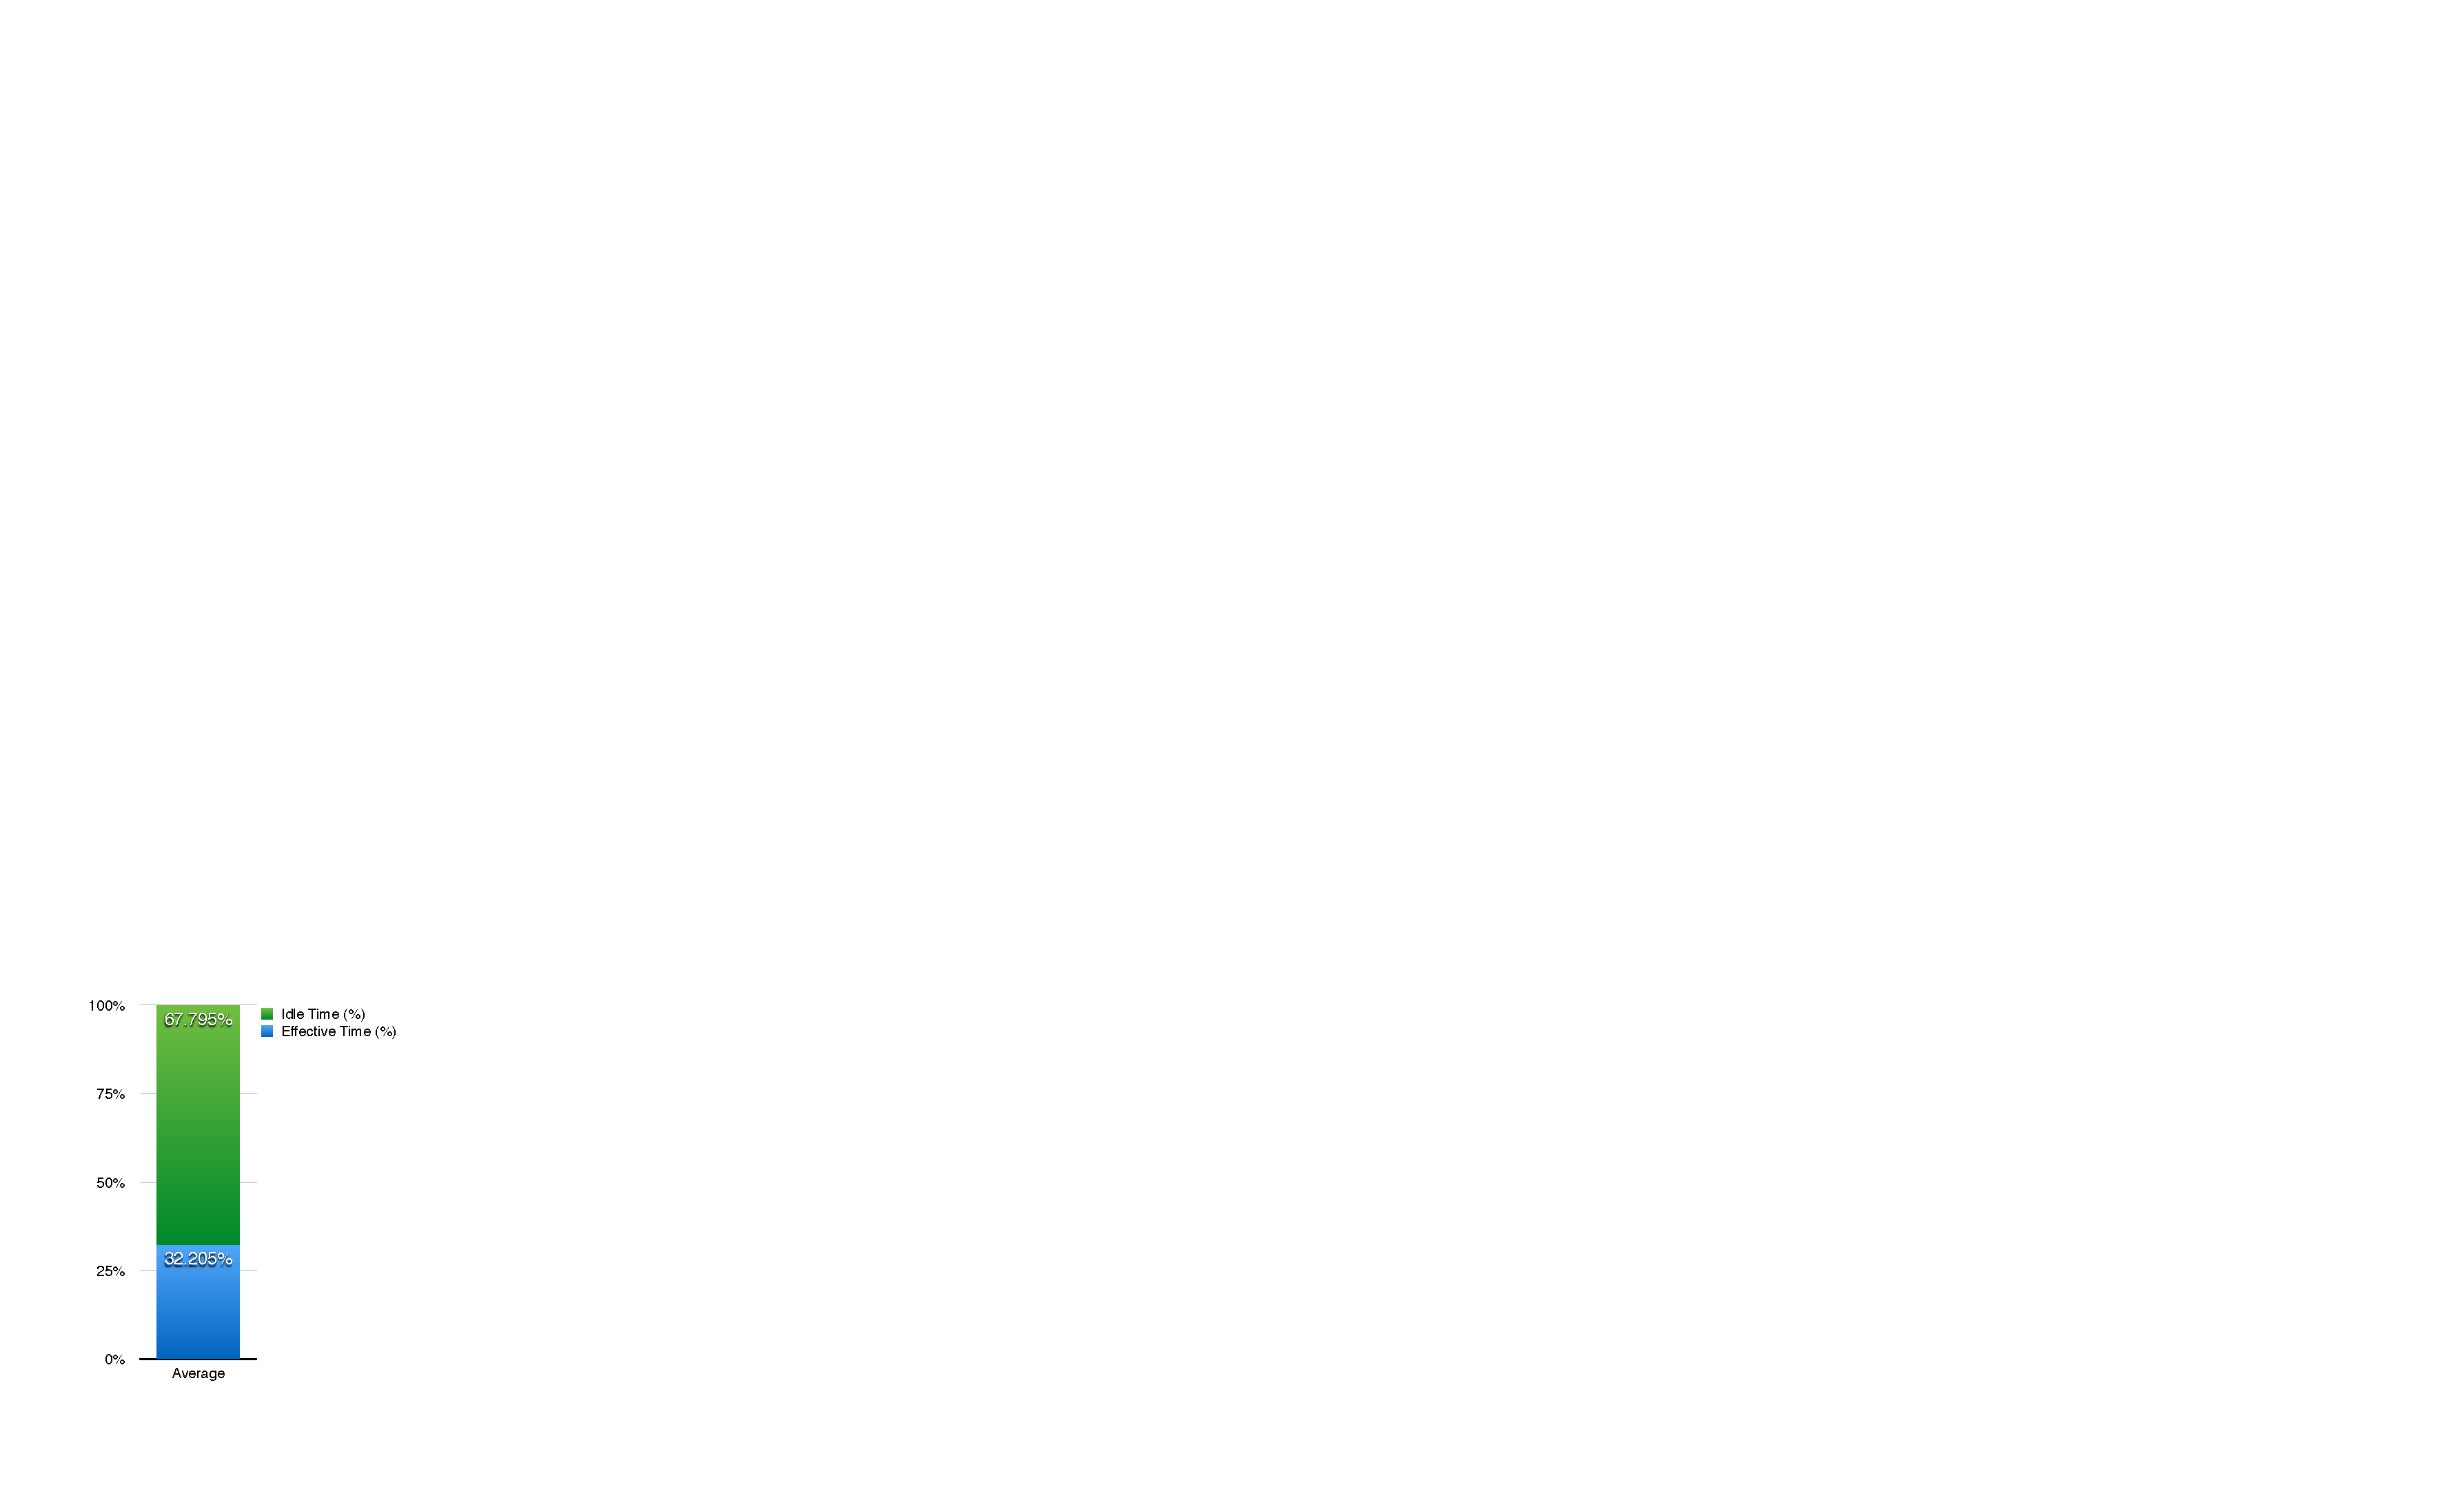
\includegraphics[width=.55\linewidth]{./figures/edge_ecspecf_breakdown}
 \caption{Half-period Event Cycle: latency breakdown.}
 \label{fig:ecspec_half}
\end{figure}

Comparing the graphs for both \textit{ECspecs} is possible to conclude that during most of the time of
an \textit{Event Cycle} the \gls{ALE} module is in an idle state (\textit{Idle Time}) - close to $\approx68\%$
in both configurations - while in the remaining time the \gls{ALE} is processing the event that was
collected (\textit{Effective Time}). Considering the duration of the \textit{ECspecs} it means that in
average when the \gls{ALE} is configured with the \textit{Baseline ECspec} the module can be in an idle
state during 7s while with the \textit{Half-period ECspec} this idle state can last for 3 seconds.

% Event Effective Time Breakdown
\textit{b) Event Effective Time Breakdown.}
Figure~\ref{fig:ecspec_effective_base} presents the time breakdown for each stage of the pipeline
when the \gls{ALE} is configured with \textit{Baseline ECspec} and in Figure~\ref{fig:ecspec_effective_half}
when it is configured with the \textit{Half-period ECspec}.

% ECSpec breakdown
\begin{figure}[ht!]
  \centering
  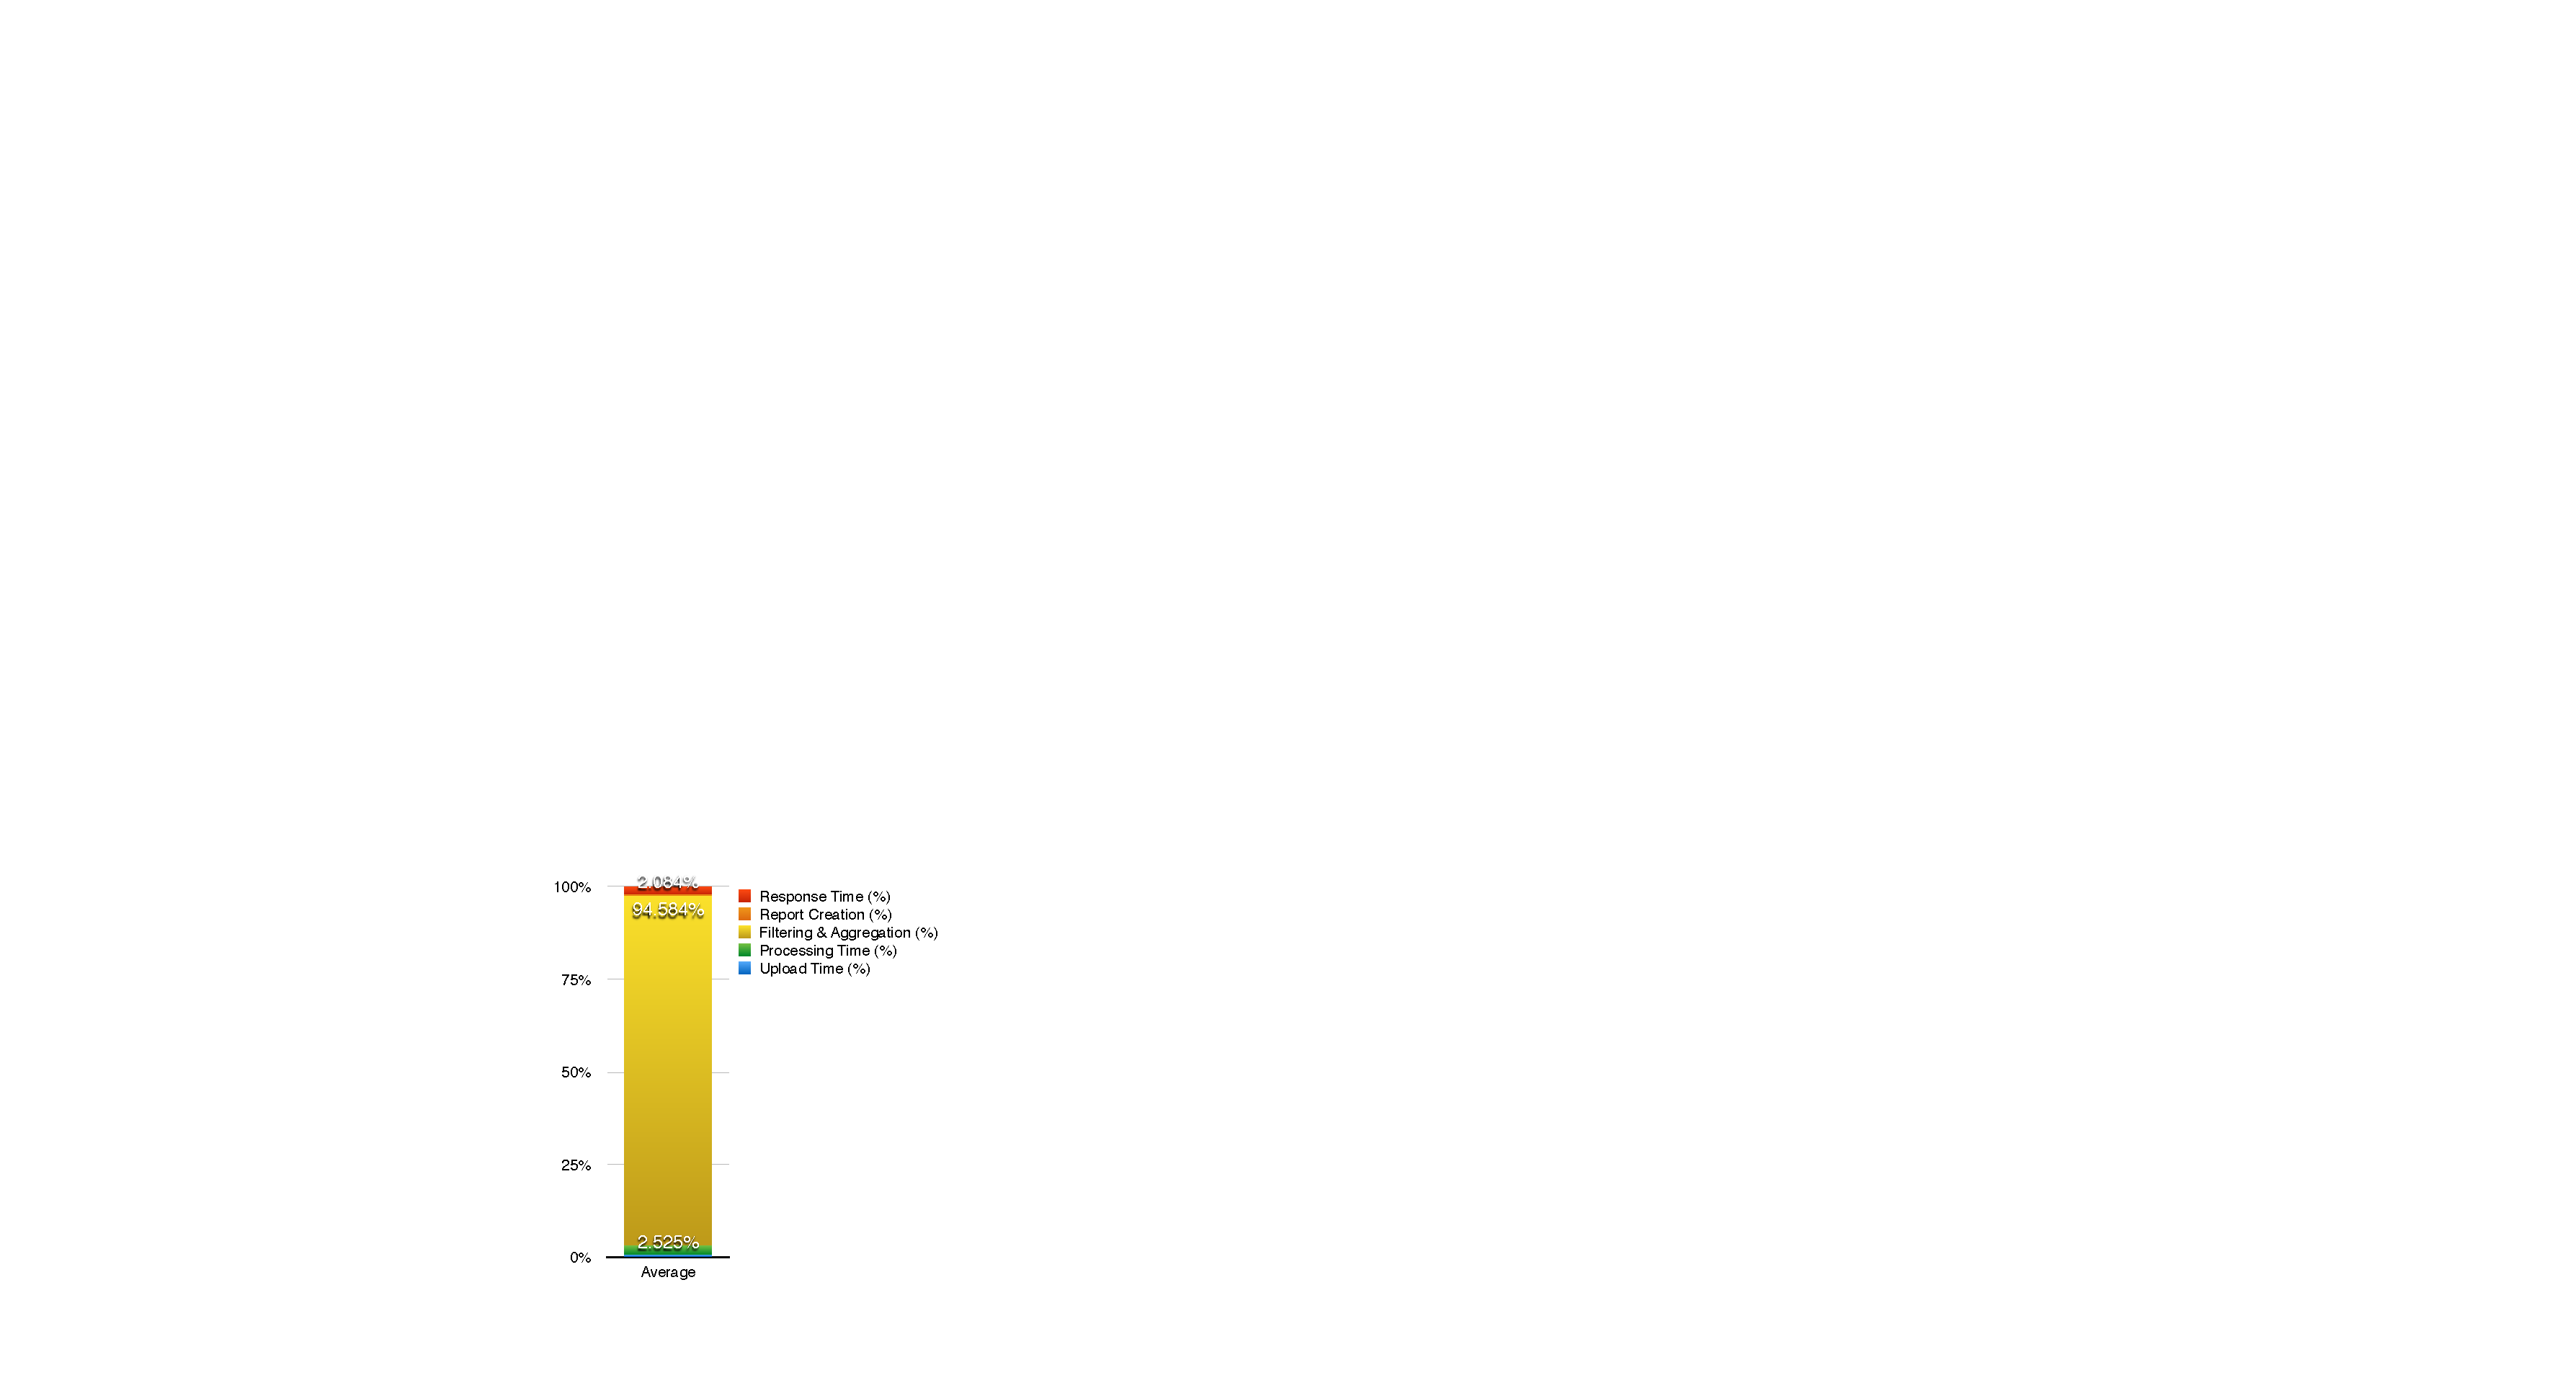
\includegraphics[height=.7\linewidth]{./figures/edge_ecspec_effective_breakdown}
  \caption{Baseline Event Cycle: event pipeline breakdown.}
  \label{fig:ecspec_effective_base}
\end{figure}

% ECSpec fast breakdown
\begin{figure}[ht!]
  \centering
  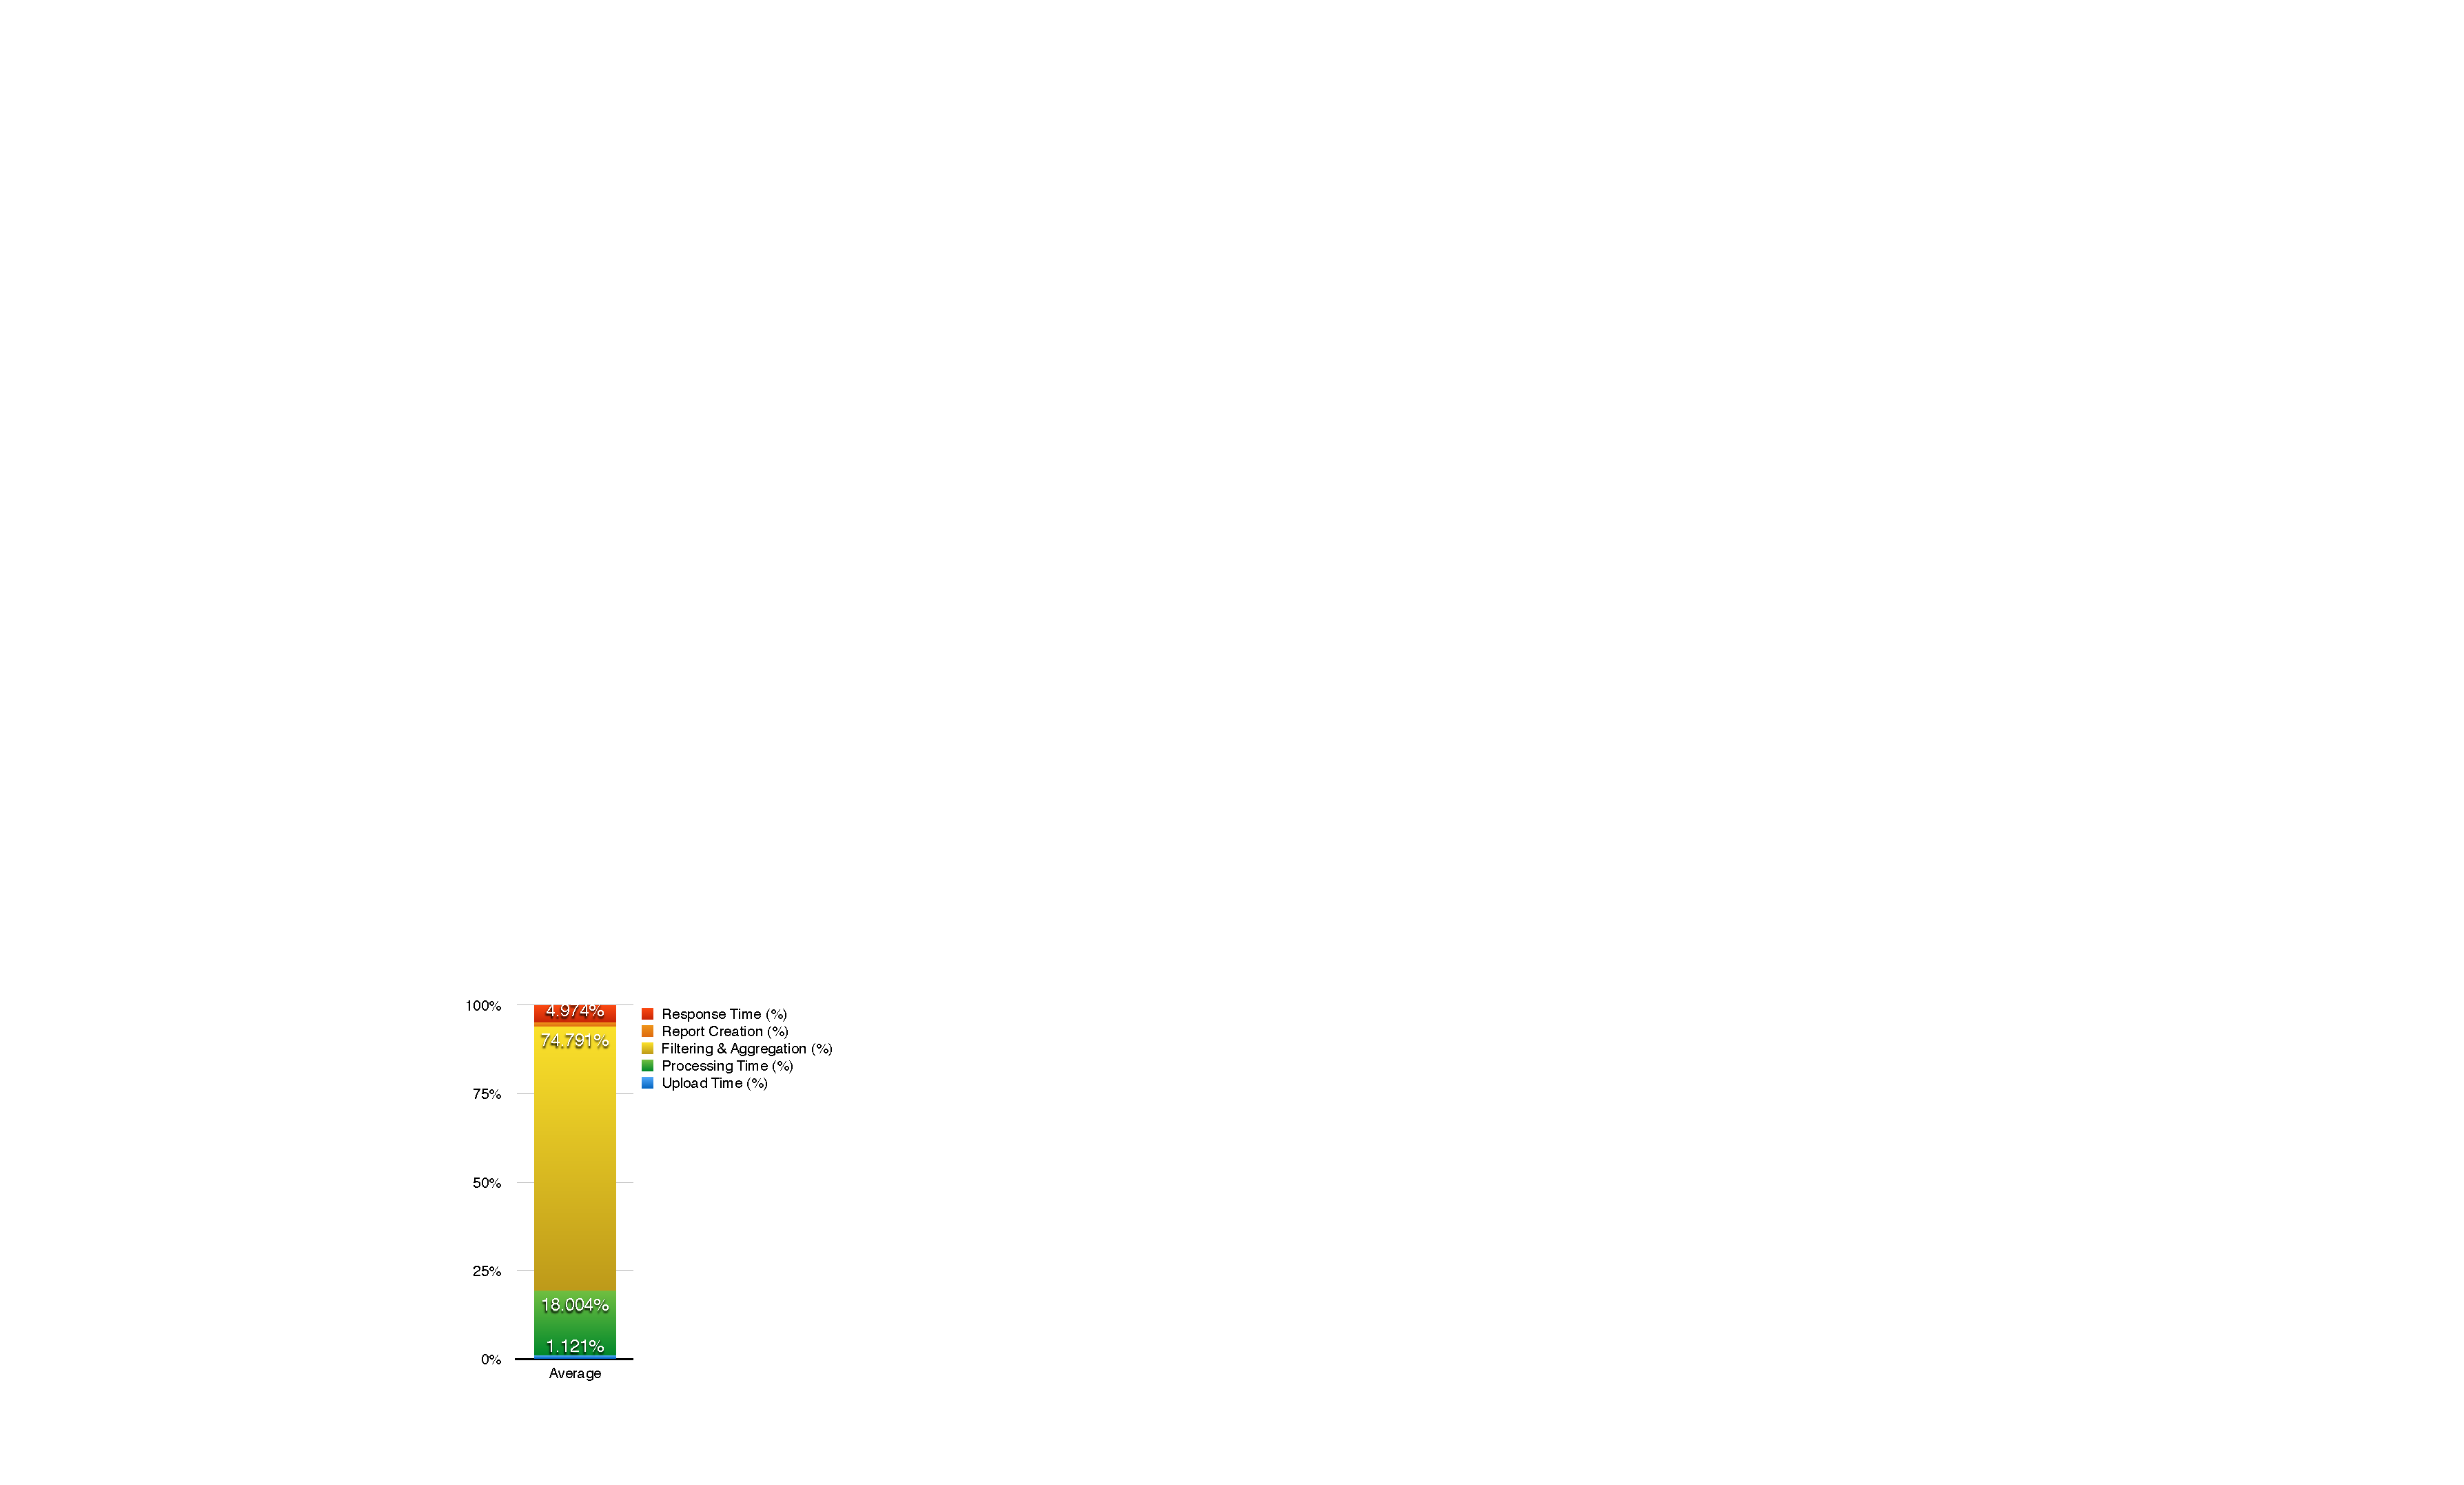
\includegraphics[width=.7\linewidth]{./figures/edge_ecspecf_effective_breakdown}
  \caption{Half-period Event Cycle: event pipeline breakdown.}
  \label{fig:ecspec_effective_half}
\end{figure}

It is possible to observe that the \textit{Fltering \& Aggregation} stage is the most time consuming
for both \textit{Event Cycle} specifications. With the \textit{Baseline ECspec} this stage occupies
close to $\approx95\%$ of the total time, while with the \textit{Half-period ECspec} this value is
close to $\approx75\%$. The reason for this difference is in the \textit{Tag Processing} stage.
With the \textit{Baseline ECspec} the time for processing the event data represents close to $\approx2.5\%$
of the total time while with the \textit{Half-period ECspec} this value is close to $\approx18\%$.
The \textit{Upload} and \textit{Response} stages together represents a small percentage of
the time spent to process the event - close to $\approx5\%$ for both specifications - while the percentage
of time to create the reports represents less than $\approx1\%$ of the total time.

\textit{c) Experiment Result.}
As in the previous experiment, in our scenario the warehouse door only will open if the \gls{ALE}
module was configured with the \textit{Half-period ECspec}, otherwise the robot will crash with
the door.

% Data storage
\subsubsection{Data Storage Performance}
\label{subs:data_storage_performance}
To evaluate the data storage performance for the Fosstrak middleware we use the data recorded with
the Rec\&Play module - which is able to record \gls{RFID} sessions that stores the events occurred
in the warehouse maintaining the order and time from the beginning of the session - were used as
base to execute the tests. The sessions were recorded in a scenario developed by Correia et. al \cite{Correia:Thesis:2014}.
In this scenario tagged a robot is moving in a closed circuit where two RFID antennas were used facing
each other. The evaluation reproduced some situations that can occur in a real smart warehouse,
such as the robot is moving with the standard speed, the robot is moving at twice of the standard
speed and two robots are moving together in the warehouse. In the performed experiments, we
simulated up to 5 readers sending events concurrently.

The obtained results show that the performance of the Fosstrak was acceptable where the maximum
value obtained for the \text{CPU Utilization} metric was close to 18$\%$ and the maximum
value obtained for the network traffic metric was close to 3.5 \gls{MB}. It is important
to point out that for this evaluation scenario, it is possible to conclude that the consumption
of computing resources increases as faster the robot moves in the warehouse.

% Discussion
\subsection{Results Analysis and Discussion}
\label{sub:results_analysis_discussion}
The obtained results show that a fog-based deployment offers better overall performance for a
smart warehouse application based in RFID technology that requires low latency interaction. However
we detected some performance issues in the behavior of the \gls{ALE} module. In particular, in the
performed experiments we detected that in most of the time the module remains in an idle state.
Regarding the data storage performance the obtained results show that Fosstrak is adequate
to process the amount of data generated in a smart warehouse.
